% Course report, aligned with implementation 66e0805 and checked-in evaluation evidence.
\documentclass[11pt,a4paper]{article}
\usepackage[margin=25mm]{geometry}
\usepackage[T1]{fontenc}
\usepackage{lmodern,tabularx,longtable,booktabs,xcolor,amsmath,graphicx,fancyhdr,pgfplots,tikz}
\usepackage{float}
\usepackage[hidelinks]{hyperref}
% Local editor compilation uses a temporary working directory. Relative images
% still take precedence when this single source is uploaded with its assets.
\graphicspath{{./}{C:/Users/User/d7065e-group2/claude/output/latex/D7065E-redrawn/}}
\pgfplotsset{compat=1.18}
\usetikzlibrary{arrows.meta,positioning,fit,backgrounds,shapes.geometric,babel}
\definecolor{serviceblue}{HTML}{DBEAFE}
\definecolor{devicegreen}{HTML}{DCFCE7}
\definecolor{infrapurple}{HTML}{EDE9FE}
% Shared diagram styles: native centimetres; never scale a TikZ picture.
\newdimen\diagramwidth
\newcommand{\checkdiagramwidth}{%
  \pgfextractx{\diagramwidth}{\pgfpointdiff
    {\pgfpointanchor{current bounding box}{west}}
    {\pgfpointanchor{current bounding box}{east}}}%
  \typeout{REPORT-DIAGRAM-WIDTH: \the\diagramwidth}%
  \ifdim\diagramwidth>15.5cm
    \PackageError{report-diagrams}{Diagram exceeds 15.5 cm}
      {Reduce spacing or split the diagram. Do not scale it.}%
  \fi
  \ifdim\diagramwidth>\linewidth
    \PackageError{report-diagrams}{Diagram exceeds linewidth}
      {Reduce spacing or split the diagram. Do not scale it.}%
  \fi}
\tikzset{
  every picture/.style={font=\small,execute at end picture=\checkdiagramwidth},
  msg/.style={-{Latex[length=2.5mm]}, thick},
  ret/.style={-{Latex[length=2.5mm]}, thick, dashed},
  act/.style={draw, thick, fill=blue!8, minimum width=2.1cm, minimum height=0.7cm, font=\small\bfseries, align=center},
  note/.style={draw, fill=yellow!15, font=\footnotesize, align=left, inner sep=3pt},
  phase/.style={font=\footnotesize\bfseries, text=darkgray, fill=white, inner sep=1pt, anchor=west},
  lbl/.style={above, font=\footnotesize, fill=white, inner sep=1pt},
  service/.style={act,fill=serviceblue},
  infrastructure/.style={act,fill=infrapurple},
  device/.style={act,fill=devicegreen},
  external/.style={act,fill=gray!12},
  frame/.style={draw=gray,dashed,rounded corners=2pt,inner sep=4pt},
  check/.style={diamond,draw,thick,fill=blue!8,aspect=2,align=center,font=\small,inner sep=2pt},
  process/.style={draw,thick,fill=serviceblue,align=center,font=\small,inner sep=5pt}
}
\newcommand{\diagramphase}[3]{%
  \draw[gray!55,thin] (0,#1) -- (#2,#1);
  \node[phase] at (0.05,#1) {#3};}
\newcommand{\diagramlegend}{\par\smallskip{\footnotesize
  Blue: project service; purple: messaging/storage/dashboard infrastructure;
  green: device adapter; grey: course/external service.\par}}
\pagestyle{fancy}\fancyhf{}
\fancyhead[L]{CO2 ventilation -- Group 2}\fancyhead[R]{D7065E -- Architecture Document}
\fancyfoot[C]{\thepage}\setlength{\headheight}{14pt}
\setlength{\emergencystretch}{3em}
\title{CO\textsubscript{2}-driven ventilation with thermal trade-off\\\large D7065E, Architecture Document}
\author{Group 2: Tobias Hanke \& Evangelos Vasilaras}
\date{11 October 2026}
\begin{document}
{\let\newpage\relax\maketitle}
\tableofcontents
\newpage
\section{Summary}
The system autonomously regulates ventilation and heating in five simulated rooms on level 0 of the A-house. Occupants generate CO\textsubscript{2}; fresh air removes it but also creates a heating demand. Separate sensor, controller and actuator processes close this feedback loop through MQTT and BuildSim. A reactive controller provides threshold-based responses, while an advisory planner uses lecture bookings to anticipate occupancy over 30 simulated minutes. The planner reads observed history, rather than physical ground truth, and its suggestions can raise the reactive ventilation request. JSONL/Parquet storage supports history, audit and evaluation; BuildSim overlays and Grafana expose the resulting conditions and decisions.

The current implementation adds 18 $^\circ$C mechanical supply air, 75\% heat recovery and separate air-handling-unit (AHU) energy accounting. Recorded final-configuration runs show a concrete trade-off: timetable planning reduced occupied lecture-room CO\textsubscript{2} exceedances from 122 to zero simulated minutes, increased lecture-room comfort from 70.2\% to 84.7\%, and raised all-room radiator-plus-AHU energy from 259.5 to 282.6 kWh. These are existing repository results from one simulated weekday, not new experiments performed for this revision. The 90\% comfort requirement remains unmet; the fika room still has exceedances, and the fixed-schedule energy baseline has not been evaluated.

\noindent\begin{tabularx}{\linewidth}{lX}\toprule Field & Value\\\midrule
Project & CO\textsubscript{2}-driven ventilation with thermal trade-off\\
Team & Group 2: Tobias Hanke; Evangelos Vasilaras\\
Scope & A109, A117, A110, A323 and A113C on level 0\\
Repository & \url{https://github.com/TobiMacaronisGit/d7065e-group2}\\
Implementation & \texttt{66e0805}; report revised 11 October 2026\\
Evidence & \protect\path{docs/results/faults.txt}, \protect\path{e3-results.md}, \protect\path{e3-summary.md} and \protect\path{train.txt} in the same results directory\\\bottomrule
\end{tabularx}

\paragraph{Changes since the proposal.}
The proposed four-to-six-room demonstration now uses five named rooms with explicit lecture/fika/office roles. Reactive control and planning are separate processes, allowing the reactive path to continue when history or planning is unavailable. MQTT implements observation and command distribution; JSONL, Parquet and DuckDB provide inspectable history without a separate database server.

The latest changes also respond to evidence. A linear occupancy model lost to persistence on a held-out date and was kept as an evaluation artifact rather than deployed. Lecture bookings now provide the primary forecast, with persistence used when no bookings or trained model are available. Replayed experiments exposed history contamination; the planner now bounds queries by its current simulated time and recent wall-clock receipt time. Initial thermal results showed zero occupied comfort, prompting the explicit supply-air, heat-recovery and radiator changes above. These refinements improve the demonstration. Newly recorded fault tests confirm late frozen-sensor detection and a failed actuator restart; pipeline scans now use bounded DuckDB buffers and serialized query execution. Recovery guarantees and model calibration remain open.

\paragraph{Revision scope and branch provenance.}
This revision checks the fetched GitHub main branch at \texttt{66e0805}, including the pipeline limiter and recorded F1/F3/F6 tests. Additional plots and the 18--24 $^\circ$C descriptive metric come from \protect\path{origin/tobias}, commit \texttt{fbb5552}, which was not merged into main at review time. These additions do not change the FR-02 acceptance band or constitute new simulation runs.

\section{Use case and building context}
\paragraph{Purpose and responsibilities.}
The use case is occupied-room air quality with a thermal and energy trade-off in the A-house. A lecture causes a rapid increase in people and CO\textsubscript{2}; ventilation dilutes the concentration, while heating must replace envelope and fresh-air losses. Advance knowledge of a booking can therefore justify ventilation and preheating before people arrive. A building manager observes the autonomous decisions, their reasons and room conditions. Occupants influence demand through presence; there is no implemented manual-override workflow or approval step for each command.

BuildSim is provided infrastructure holding room geometry, equipment, occupancy, sensor values and reached actuator states, with a browser-based 3D view. The course occupancy simulator supplies people, lecture bookings and the simulated clock. The project supplies room physics, simulated devices, control, planning, history and presentation integration. BuildSim is shared state, not the project's physical simulator or decision maker.

\paragraph{Rooms and scenario.}\mbox{}\par
\noindent\begin{tabularx}{\linewidth}{llrrX}\toprule Room & Role & Area (m$^2$) & Volume (m$^3$) & Demand pattern\\\midrule
A109 & Lecture & 188 & 564 & Scheduled class arrivals\\
A117 & Lecture & 214 & 642 & Several scheduled classes\\
A110 & Fika & 124 & 372 & Unscheduled shared-space occupancy\\
A323 & Office & 17 & 51 & Small-room occupancy\\
A113C & Office & 16 & 48 & Small-room occupancy\\\bottomrule\end{tabularx}
All rooms use a 3-m model height and level-qualified identities such as \protect\path{level0/A109}. The one-shot seed process overrides occupancy-simulator roles so lectures occur in the selected rooms. This concentrates useful activity in the demonstration area and narrows how representative its results are.

The recorded evaluation uses simulated Wednesday 21 October 2026, 07:30--18:00, at 60 simulated seconds per wall second. A109 is booked 08:15--10:00 for 101 students; A117 has bookings at 10:15--12:00, 13:15--15:00 and 15:15--17:00 for 97, 115 and 102 students. The simulator models early student and lecturer arrival. A110 and the offices have no lecture bookings, so their planner normally uses persistence. Fault and crash evidence is assessed separately from weekday performance; recorded F1/F3/F6 results are included in the test section.

\paragraph{Integration boundary.}
Physics reads occupancy and reached actuator states from BuildSim. Sensors sample physics, add lag/noise/fault effects, and publish observations to MQTT and BuildSim. The occupancy counter counts BuildSim persons. Control consumes observed MQTT inputs and publishes commands; actuators validate them and write their reached states to BuildSim. The planner reads observed history and bookings. Viewer alone updates room layers and alerts; Grafana reads the history API. The intended separation of physical truth from decisions is a code convention on the shared lab network, not a network access restriction.

\section{Requirements}
Requirements retain the repository IDs and distinguish simulated time (sim-min) from real elapsed time (s wall). Table~\ref{tab:req} traces the acceptance criteria to the architecture and verification plan. A configuration setting is not treated as a measured guarantee.
{\small\begin{longtable}{p{19mm}p{83mm}p{42mm}}
\caption{Requirements and traceability, from \protect\path{docs/requirements.md}.}\label{tab:req}\\
\toprule ID & Acceptance criterion & Design / verification\\\midrule\endfirsthead
\toprule ID & Acceptance criterion & Design / verification\\\midrule\endhead
FR-01 & Occupied-room CO\textsubscript{2} returns below 1000 ppm within 10 sim-min after exceeding it. & Reactive rules, ventilation; S1.\\
FR-02 & At least 90\% of occupied sim-min are within 20--24 $^\circ$C over a weekday. & Setpoints and physics; S1.\\
FR-03 & Within 15 sim-min of emptying, ventilation reaches its configured minimum target and heating target is 17 $^\circ$C. & Setback rules; S1.\\
FR-04 & Forecasting reduces occupied CO\textsubscript{2} exceedance minutes by at least 50\% relative to reactive-only on the same day/seed. & Planner; E3, E5.\\
FR-05 & Decisions contain reasons and inputs and can be retrieved from history. & Decision schema and pipeline; audit inspection.\\
NFR-01 & Median per-room decision interval is at most 60 s wall under five-room load. & Five-second control loop; E4.\\
NFR-02 & After a process crash/restart, correct commands resume within 60 s wall without unsafe intervening commands. & Process isolation, reconnect/restart; F3/F4.\\
NFR-03 & No actuator target changes more than once per 5 sim-min, except SAFETY. & Hysteresis/dwell; E2.\\
NFR-04 & Weekday modelled heating energy is no greater than a fixed-schedule baseline. & Occupancy setback; E1.\\
NFR-05 & Frozen CO\textsubscript{2} is detected within 10 sim-min; control continues from occupancy in DEGRADED mode. & Quality classifier; F1/F2.\\
NFR-06 & Following a BuildSim restart, devices re-register and readings resume within 60 s wall without reseeding. & Device self-registration; F5.\\
NFR-07 & A 60-s-wall pipeline outage loses no readings. & QoS 1 and persistent consumer session; F3/F4.\\
REG-01 & Every ventilation command is at least the configured minimum, in every mode. & Final clamp; rule review.\\
SAF-01 & Reject commands with an incorrect issuer, out-of-range target or wall age over 120 s. & Actuator validation; F6.\\\bottomrule
\end{longtable}}
REG-01 names a configurable invariant; the minimum is currently zero, so it does not establish compliance with an external ventilation standard. SAF-01 checks a literal issuer string, not authenticated identity. Section~\ref{sec:results} reports evidence and gaps against these criteria.

\paragraph{Temperature target and guidance.}
FR-02's 20--24 $^\circ$C band is a project comfort target, not an established legal requirement. The newer branch additionally reports time within 18--24 $^\circ$C. Swedish public-health guidance HSLF-FS 2024:10 gives operative-temperature guideline values of 18 $^\circ$C minimum (20 $^\circ$C for sensitive groups) and 24 $^\circ$C maximum in autumn, winter and spring. Operative temperature includes surrounding-surface radiation; this project models air temperature only. The additional metric therefore provides context, not a regulatory-compliance finding, and does not replace FR-02.
Source: \href{https://www.folkhalsomyndigheten.se/contentassets/1c28701a4c8f49cabce85e3bb65695dc/hslf-fs-2024-10.pdf}{Folkh\"alsomyndigheten, HSLF-FS 2024:10, Tables 1--3}.

\section{Architecture}
\subsection{Context diagram (C4 Level 1)}
Figure~\ref{fig:context} incorporates the updated context view in \protect\path{docs/diagrams/context.d2}. Arrows show information flow; dashed REST/browser responses flow from the responding provider to the consumer, while solid arrows show messages or writes.
\begin{figure}[H]\centering
\begin{tikzpicture}
\node[external,text width=3cm] (people) at (1.8,0) {Occupants};
\node[external,text width=3cm] (manager) at (12.6,0) {Building manager};
\node[external,text width=3cm,minimum height=1.8cm] (occ) at (1.8,-3.2)
 {occupancysim\\\normalfont People, bookings, clock};
\node[service,text width=4cm,minimum height=2.2cm] (sys) at (7.2,-3.2)
 {Ventilation and\\climate control\\\normalfont Five rooms on level 0\\Physics, devices, control,\\planning and history};
\node[external,text width=3cm,minimum height=2.2cm] (bs) at (12.6,-3.2)
 {BuildSim\\\normalfont Shared occupancy,\\values, reached states;\\browser 3D view};
\draw[msg] (people.south) -- node[lbl,xshift=0.9cm]{presence} (occ.north);
\draw[ret] (occ.north east) -- (3.45,-1.6) -- node[lbl]{clock + bookings} (5.03,-1.6) -- (sys.north west);
\draw[ret] (bs.west) -- node[lbl]{room inputs} (sys.east);
\draw[msg] (sys.south east) -- (8,-4.9) -- node[lbl]{values / states / view} (11.8,-4.9) -- (bs.south west);
\draw[msg] (occ.south) -- (1.8,-5.65) -- node[lbl]{occupancy + entities} (13.4,-5.65) -- (bs.south east);
\draw[msg] (sys.north) -- (7.2,-1.1) -- node[lbl]{history / decisions} (12.6,-1.1) -- (manager.south);
\draw[ret] (bs.east) -- (14.55,-3.2) -- (14.55,0.9) -- node[lbl]{3D view} (12.6,0.9) -- (manager.north);
\node[note,text width=13.6cm] at (7.2,-6.9)
 {\textbf{Scope and boundary.} A109/A117: lectures; A110: fika; A323/A113C: offices.\\
 No manual override. Shared lab host/network; truth separation is a code convention.\\
 Balance CO$_2$, thermal comfort and radiator + AHU heating energy.\\
 Manager views include health; BuildSim supplies 3D conditions and alerts. Clock factor: 60.};
\end{tikzpicture}
\diagramlegend
\caption{System context: all seven information flows from \texttt{context.d2}. Solid arrows show messages/writes; dashed arrows show read or browser responses. Room inputs are occupancy and reached actuator states. Writes include sensor values, reached states, room layers and alerts.}\label{fig:context}
\end{figure}

\subsection{Container diagram (C4 Level 2)}
Figures~\ref{fig:containers} and~\ref{fig:containers-support} incorporate \protect\path{docs/diagrams/container.d2} and separates observation, decisions and actuation into processes. Green boxes group device instances; blue boxes are project services; purple boxes are messaging, storage or dashboard infrastructure; grey boxes are provided services. Grouping ten sensors or actuators in a box does not imply a shared process.
\begin{figure}[H]\centering
\begin{tikzpicture}
\node[service,text width=3cm] (phy) at (1.95,0) {physics\\\normalfont Python; 8090\\CO$_2$, heat, energy};
\node[external,text width=3cm] (bs) at (7.35,0) {BuildSim\\\normalfont Go; 9090\\Occupancy, states};
\node[external,text width=3cm] (occ) at (12.75,0) {occupancysim\\\normalfont Go; 8081\\People, clock,\\bookings};
\node[device,text width=3cm] (sen) at (1.95,-3.5) {sensor-* $\times10$\\\normalfont Python; 2 s wall\\CO$_2$/temperature};
\node[device,text width=3cm] (cnt) at (12.75,-3.5) {occupancy\_\\counter\\\normalfont Python; 2 s wall\\Shared container};
\node[infrastructure,text width=3cm] (mq) at (7.35,-6.5) {broker\\\normalfont Mosquitto\\MQTT 1883; QoS 1\\Retained targets};
\node[device,text width=3cm] (act) at (1.95,-9.4) {actuator-* $\times10$\\\normalfont Python; vent / heat\\Validate and move};
\node[service,text width=3cm] (ctl) at (12.75,-9.4) {control\\\normalfont Python; 8091\\Every 5 s wall};
\draw[ret] (bs.west) -- node[lbl]{room inputs} (phy.east);
\draw[msg] (occ.west) -- node[lbl]{occupancy} (bs.east);
\draw[ret] (phy.south) -- node[lbl,xshift=1cm]{room truth} (sen.north);
\draw[ret] (bs.south east) -- node[lbl]{persons} (cnt.north west);
\draw[msg] (sen.east) -- node[lbl]{observations} (6.75,-3.5) -- (mq.north west);
\draw[msg] (cnt.west) -- node[lbl]{head counts} (7.95,-3.5) -- (mq.north east);
\draw[msg] (mq.east) -- node[lbl]{inputs + plans} (12.75,-6.5) -- (ctl.north);
\draw[msg] (ctl.north west) -- (11,-8.1) -- node[lbl]{cmd / decision} (8.1,-8.1) -- (mq.south -| 8.1,0);
\draw[msg] (mq.west) -- node[lbl]{commands} (1.95,-6.5) -- (act.north);
\draw[msg] (act.east) -- (4.15,-9.4) -- (4.15,-8.1) -- node[lbl]{state + fault} (6.7,-8.1) -- (mq.south -| 6.7,0);
\draw[msg] (act.west) -- (-0.25,-9.4) -- (-0.25,2) -- node[lbl]{reached states} (7.35,2) -- (bs.north);
\draw[msg] (sen.west) -- (0.1,-3.5) -- (0.1,1.1) -- node[lbl]{display values} (6.7,1.1) -- (bs.north west);
\draw[ret] (occ.north) -- (12.75,2.9) -- node[lbl]{simulated clock} (1.95,2.9) -- (phy.north);
\end{tikzpicture}
\diagramlegend
\caption{Container view, panel A: the live feedback loop. Numbers are HTTP host ports except broker's MQTT port. Each device group represents ten independent Compose services. Panel B completes the same inventory. Short labels retain the \texttt{container.d2} contracts; state reports carry target, motion and fault.}\label{fig:containers}
\end{figure}

\begin{figure}[H]\centering
\begin{tikzpicture}
\node[infrastructure,text width=3cm] (mq) at (7.3,0) {broker\\\normalfont Same as panel A};
\node[infrastructure,text width=3cm] (pipe) at (1.8,-3) {pipeline\\\normalfont Python / DuckDB\\HTTP 8092\\JSONL / Parquet};
\node[service,text width=3cm] (plan) at (12.8,-3) {planner\\\normalfont Python / NumPy\\HTTP 8093\\Every 10 s wall};
\node[service,text width=3cm] (view) at (1.8,-6) {viewer\\\normalfont Python; HTTP 8094\\Layers + alerts};
\node[infrastructure,text width=3cm] (graf) at (7.3,-6) {grafana\\\normalfont HTTP 3000; Infinity\\Historical JSON};
\node[external,text width=3cm] (occ) at (12.8,-6) {occupancysim\\\normalfont Same as panel A};
\node[external,text width=3cm] (bs) at (7.3,-9) {BuildSim\\\normalfont Same as panel A};
\node[service,text width=3cm] (seed) at (12.8,-9) {seed\\\normalfont One-shot setup\\No published port};
\draw[msg] (mq.south west) -- node[lbl]{archive events} (pipe.north east);
\draw[ret] (pipe.east) -- node[lbl]{observed history} (plan.west);
\draw[msg] (plan.north west) -- node[lbl]{retained Plan} (mq.south east);
\draw[msg] (mq.west) -- node[lbl]{live events} (-0.1,0) -- (-0.1,-6) -- (view.west);
\draw[ret] (pipe.south east) -- node[lbl]{query JSON} (graf.north west);
\draw[ret] (occ.north) -- node[lbl,xshift=-1.2cm]{clock + bookings} (plan.south);
\draw[msg] (view.south east) -- node[lbl]{layers + alerts} (bs.north west);
\draw[msg] (seed.west) -- node[lbl]{register} (bs.east);
\draw[msg] (seed.north) -- node[lbl,xshift=1cm]{room roles} (occ.south);
\node[note,text width=13.6cm] at (7.3,-11)
 {\textbf{Compose inventory across panels A and B:} 10 sensors + 10 actuators + 10 shared\\
 containers = 30 continuing containers, plus one-shot seed. Repeated boxes are references.\\
 Shared: broker, grafana, BuildSim, occupancysim, physics, occupancy\_counter, control,\\
 planner, pipeline and viewer. Devices each run separately; the counter is one shared process.};
\end{tikzpicture}
\diagramlegend
\caption{Container view, panel B: planning, history, presentation and setup. The two panels preserve all 20 runtime edges in \texttt{container.d2}. Seed and its two setup writes are added from Compose and \texttt{scripts/seed.py}; seed is omitted from the D2 runtime view.}\label{fig:containers-support}
\end{figure}
Control consumes live MQTT without waiting for disk or history queries. Planner depends on history; its failure removes new advice while reactive decisions continue. Physics is observed through sensors, and only actuators write reached states. This preserves a meaningful feedback path rather than treating a command as an instantaneous physical change.
The short labels retain the following contracts from \texttt{container.d2}: room inputs are occupancy plus reached actuator states; observations are CO$_2$/temperature and head counts; actuator state reports carry state, target, motion and fault. Control publishes changed-target commands and decisions/reasons. Pipeline archives \protect\path{bldg/#} and \protect\path{sys/health/#}; history requests use \texttt{until} and \protect\path{max_age_s}. Viewer replaces full room-layer/alert arrays. Sensors use lag, noise and fault effects; physics uses 18 $^\circ$C supply, 75\% heat recovery and HTTP radiator/AHU counters. Pipeline compacts every 300 s wall; planner selects the lowest level with predicted peak below 900 ppm across 30 sim-min. Grafana 12.3.0 uses Infinity 4.1.1.

Other services also use the shared SimClock client. The rejected learned model is not deployed, although its fallback branch remains in code. Radiator/AHU counters are HTTP truth fields rather than an automatically archived MQTT stream. The one-shot seed is shown separately from continuing runtime flows in the setup panel. It registers equipment and configures room roles; it is not a continuing container.

\subsection{Component diagram (C4 Level 3)}
The control process is the most useful internal view because it owns precedence and mode selection (Figure~\ref{fig:components}). Its subscribers update observations and plans; per-room controller state keeps repeated-value history, previous target and change time. Quality assessment selects a mode, rules merge reactive demand with acceptable advice, and final clamps precede publication. HTTP exposes the latest decisions for inspection.
\begin{figure}[H]\centering
\begin{tikzpicture}
\node[infrastructure,text width=3.8cm] (mq) at (7.2,0) {MQTT broker\\\normalfont Observations / plans in\\Commands / decisions out};
\node[service,text width=3.6cm] (sub) at (2.1,-2.7) {Bus callbacks\\\normalfont Decode; route by room/type};
\node[service,text width=3.6cm] (cache) at (7.2,-2.7) {Room state/cache\\\normalfont Readings, plan, prior target};
\node[service,text width=3.6cm] (quality) at (12.3,-2.7) {Quality assessment\\\normalfont Age and repeated CO$_2$};
\node[service,text width=3.6cm] (pub) at (2.1,-5.5) {Publisher + API\\\normalfont Commands on change\\Every decision with reason};
\node[service,text width=3.6cm] (clamp) at (7.2,-5.5) {Output constraints\\\normalfont Downward dwell / margin\\Final minimum clamp};
\node[service,text width=3.6cm] (rules) at (12.3,-5.5) {RoomController\\\normalfont Mode, thresholds,\\plan precedence};
\node[external,text width=7cm] (cfg) at (7.2,-8.2) {Configuration + SimClock\\\normalfont Thresholds, intervals, shared simulated time};
\draw[msg] (mq.west) -| (sub.north);
\draw[msg] (sub) -- (cache);
\draw[msg] (cache) -- (quality);
\draw[msg] (quality) -- (rules);
\draw[msg] (rules) -- (clamp);
\draw[msg] (clamp) -- (pub);
\draw[msg] (pub.west) -- (-0.15,-5.5) -- (-0.15,1.1) -- node[lbl]{commands / decisions} (7.2,1.1) -- (mq.north);
\draw[msg] (cfg.north) -- (clamp.south);
\draw[msg] (cfg.east) -| (rules.south);
\begin{scope}[on background layer]
\node[frame,fit=(sub)(cache)(quality)(pub)(clamp)(rules)] {};
\end{scope}
\node[phase] at (0.2,-6.7) {control container [Python]};
\end{tikzpicture}
\caption{Components within control, checked against \protect\path{control/main.py} and \protect\path{control/rules.py}; there is no component D2 source. Boxes are logical responsibilities: quality and constraints are stages inside RoomController. Configuration and SimClock are logical inputs; general range and drift detection remain absent.}\label{fig:components}
\end{figure}

\subsection{Design decisions and alternatives}
{\small\begin{longtable}{p{39mm}p{45mm}p{60mm}}\toprule Choice & Alternative & Reason and cost\\\midrule\endhead
Separate reactive control and advisory planner & One learned controller or joint optimiser & Threshold precedence remains inspectable and history failure does not stop reactive control; no joint optimum is obtained.\\
MQTT commands/observations; REST queries & REST polling for all exchanges & Fan-out and retained latest targets simplify consumers; broker availability, duplication and stale retained values require care.\\
One process per simulated device & One aggregate device service & Enables isolated faults and crashes; twenty device containers increase resource use.\\
JSONL + Parquet/DuckDB & Time-series database server & Inspectable raw evidence and portable offline analysis; scans and full compaction grow with history.\\
Timetable forecasting with persistence fallback & Deploy the fitted linear model & Held-out linear MAE exceeded persistence at every horizon; bookings anticipate class arrivals but assume attendance.\\
Well-mixed room model with explicit AHU heating & Fixed traces or detailed CFD & Actuation changes later observations and energy cost is visible; parameters remain uncalibrated and spatial effects are absent.\\\bottomrule\end{longtable}}

\section{Interfaces and data contracts}
\paragraph{Communication choices.}
MQTT publish--subscribe distributes observations to control, storage and presentation without a separate request to each consumer. Control also publishes actuator commands through MQTT, keeping command validation and application in independent device processes. REST provides request--response for truth sampling, historical queries, registration and every project call into BuildSim. BuildSim provides the browser's live 3D view, including its own WebSocket transport; this project does not implement that transport. MQTT supports fan-out and short consumer outages (NFR-02/07), while REST makes queries and device-write failures explicit. The trade-off is a shared broker plus delivery and freshness handling at consumers.

\paragraph{Identity, types and time.}
Messages are UTF-8 JSON. MQTT values and targets are numbers; BuildSim sensor values and actuator states are strings. Room-scoped payloads carry string fields \texttt{level}, \texttt{room}, \protect\path{sim_ts} and \texttt{ts}. Wall-clock ISO-8601 \texttt{ts} measures command age and transport delay; simulated \protect\path{sim_ts} measures model time, freshness and forecast horizons. Sequence counters are process-local integers and restart with the process. Producer dataclasses specify the contract, but a universal runtime schema validator is not implemented.

Let \texttt{B} denote \protect\path{bldg/<level>/<room>}. All topics use QoS 1: duplicates are possible. Table entries describe configured publication intervals rather than measured guarantees.
{\small
\begin{longtable}{p{57mm}p{53mm}p{34mm}}
\toprule Topic & Direction and payload & Rate; retention\\\midrule\endhead
\protect\path{B/sensor/<type>} & Sensor/counter to broker; SensorReading & 2 s wall; no\\
\protect\path{B/actuator/<kind>/cmd} & Control to actuator; ActuatorCommand & Changed target; yes\\
\protect\path{B/actuator/<kind>/state} & Actuator to subscribers; ActuatorState & On motion/report; yes\\
\protect\path{B/plan} & Planner to control; Plan & 10 s wall loop; yes\\
\protect\path{B/decision} & Control to history/viewer; Decision & 5 s wall loop; no\\
\protect\path{sys/health/<service>} & Service/broker to subscribers; Health & Service-dependent; yes\\
\protect\path{sys/fault/<device-id>} & Operator to device; mode object & On injection; no by script\\\bottomrule
\end{longtable}}
Sensor types are \texttt{co2}, \texttt{temperature} and \texttt{occupancy}; actuator kinds are \texttt{vent} and \texttt{heat}. Actuator states are reported while moving and periodically after roughly ten wall seconds without a report. Applying a repeated valid target is idempotent. Retention restores a latest value, not a complete history.

\paragraph{Payload schemas.}
Room-scoped messages include the common fields above plus:
\begin{description}
\item[SensorReading.] String fields: \protect\path{sensor_id}, \texttt{type}, \texttt{unit}, \texttt{quality}. Numeric field: \texttt{value}; integer: \texttt{seq}. Units are ppm, degrees Celsius and persons. Quality defaults to \texttt{ok}; device faults also appear in health and are not universally encoded as suspect readings.
\item[ActuatorCommand.] Strings: \protect\path{actuator_id}, \texttt{kind}, \texttt{reason}, \protect\path{issued_by}. Number: \texttt{target}; integer: \texttt{seq}. Vent targets are in $[0,3]$; heat setpoints are in $[10,26]$ $^\circ$C. A device checks its own ID, the literal issuer \texttt{control}, numeric range and a parseable wall timestamp no more than 120 seconds old. Duplicate targets can be accepted; future timestamps and sequence ordering are not checked. The issuer string is not authenticated identity.
\item[ActuatorState.] Strings: \protect\path{actuator_id}, \texttt{kind}, \texttt{fault}; numbers: \texttt{state}, \texttt{target}; boolean: \texttt{moving}. Fault is none/stuck/slow. Its simulated timestamp is inherited from the last command, possibly empty at startup; its wall timestamp dates each publication.
\item[Plan.] Integer \protect\path{horizon_min}; six-number array \protect\path{occupancy_forecast}; number \protect\path{co2_forecast_max_ppm}; integer \protect\path{suggested_vent}; number \protect\path{suggested_setpoint_c}; string \protect\path{model_version}. Forecast points correspond to 5, 10, 15, 20, 25 and 30 sim-min. The maximum concentration is predicted at the suggested ventilation level.
\item[Decision.] String \texttt{state}, integer \texttt{vent}, number \protect\path{setpoint_c}, string \texttt{reason}, object \texttt{inputs}. States are NORMAL, DEGRADED, SAFETY and NO\_DATA. Inputs record CO\textsubscript{2}, its quality, temperature, occupancy and accepted plan ventilation; unavailable values can be null. The reason supports auditability (FR-05).
\end{description}
Health is not room-scoped: it contains service/status/detail strings and wall \texttt{ts}; status is ok/degraded/down. The broker's down last will contains only service and status. A fault request contains a string \texttt{mode}. Sensors accept none/stuck/offline/drift and actuators accept none/stuck/slow.

\paragraph{Example messages.}
These illustrate wire formats, not recorded experiments. A CO\textsubscript{2} observation on \protect\path{bldg/level0/A109/sensor/co2} and a command on \protect\path{bldg/level0/A109/actuator/vent/cmd} are:
{\small\begin{verbatim}
{"sensor_id":"A109-co2","level":"level0","room":"A109",
 "type":"co2","unit":"ppm","value":1042.0,"seq":381,
 "quality":"ok","sim_ts":"2026-10-21T10:15:00+00:00",
 "ts":"2026-10-10T08:00:00.000+00:00"}

{"actuator_id":"A109-vent","level":"level0","room":"A109",
 "kind":"vent","target":2.0,"reason":"CO2 above 1000 ppm",
 "issued_by":"control","seq":52,
 "sim_ts":"2026-10-21T10:15:00+00:00",
 "ts":"2026-10-10T08:00:00.500+00:00"}
\end{verbatim}}

\paragraph{HTTP interfaces.}
Project containers listen on port 8000. Host ports are physics 8090, control 8091, pipeline 8092, planner 8093 and viewer 8094; BuildSim uses 9090 and occupancysim 8081. Table~\ref{tab:http} specifies calls made or exposed by the project. Successful service queries return JSON; errors and special ownership semantics are noted explicitly.
{\small
\begin{longtable}{p{27mm}p{63mm}p{54mm}}
\caption{HTTP contracts.}\label{tab:http}\\\toprule Owner & Method / route & Payload and semantics\\\midrule\endfirsthead
\toprule Owner & Method / route & Payload and semantics\\\midrule\endhead
physics & GET \protect\path{/rooms}; GET \texttt{/rooms/\{room\}} & Truth array or one snapshot; unknown room gives 404. Sensors poll the single-room route.\\
control & GET \protect\path{/decisions} & Room-name map of latest Decision.\\
planner & GET \protect\path{/plans} & Room-name map of latest Plan.\\
pipeline & GET \protect\path{/history} & Parameters room/type, minutes=120, level=level0; optional until and max\_age\_s; rows sorted by simulated time.\\
pipeline & GET \protect\path{/query?sql=...} & URL-encoded SQL; at most 10,000 objects; 400 for disallowed prefix, 500 for other query errors.\\
pipeline & GET \protect\path{/stats}; POST \protect\path{/compact} & Process counters/compaction metadata; rebuild Parquet and return source counts.\\
Project services & GET \protect\path{/healthz} & Service/status plus service-specific fields; coverage of dependencies varies.\\
BuildSim & GET \protect\path{/api/occupancy} & Room-keyed objects with persons arrays; counter and physics read them.\\
BuildSim & GET \texttt{/api/actuators/\{id\}} & Actuator record with string-valued reached state; physics polls it.\\
BuildSim & PUT \texttt{/api/sensors/\{id\}/value} & Body contains data\_type=text and string value; device write gives 404 before registration.\\
BuildSim & PUT \texttt{/api/actuators/\{id\}/state} & Body contains string state; actuator is the writer.\\
BuildSim & POST \protect\path{/api/equipment/bulk} & Array of equipment records; idempotent creation and device re-registration after 404.\\
BuildSim & PUT \protect\path{/api/room-layers}; PUT \protect\path{/api/alerts} & Full arrays replace collections; viewer is the single writer.\\
occupancysim & GET \protect\path{/api/state} & sim.clock.time/factor/running supply the clock; sim.lectures supplies bookings.\\
occupancysim & GET / PUT \protect\path{/api/config} & Configuration object; seed updates room\_roles.\\\bottomrule
\end{longtable}}
The truth snapshot includes room/level/time, CO\textsubscript{2} ppm, temperature, occupants, reached ventilation, heating setpoint, heater watts, outdoor temperature and dependency flags. The legacy \protect\path{energy_kwh} is radiator-only energy; \protect\path{ahu_w} and \protect\path{ahu_kwh} describe supply-air heating, and \protect\path{total_kwh} is radiator plus AHU energy. These HTTP truth fields are not automatically an archived MQTT energy stream.

Each booking in \texttt{sim.lectures} has string \texttt{level}/\texttt{room} and numeric \texttt{start}, \texttt{end}, \texttt{students}, \texttt{seats}; start/end are minutes of the simulated day. For example, a booking object can be:
{\small\begin{verbatim}
{"level":"level0","room":"A109","start":495,"end":600,
 "students":101,"seats":94}
\end{verbatim}}
Registered students and seats are distinct; the timetable forecast does not clip registration to seats. The occupancy map is reduced by counting each room's persons array. Equipment registration records contain ID, name, type, category, room, level, status and nested sensor/actuator records; BuildSim state fields are text, as defined in \protect\path{common/buildsim.py}.

History rows contain \protect\path{sim_ts}, \texttt{ts}, \texttt{value}, \texttt{seq} and \texttt{quality}. A replay-safe request is, for example:
{\small\begin{verbatim}
GET /history?room=A109&type=co2&minutes=10&level=level0
    &until=2026-10-21T10:15:00%2B00:00&max_age_s=70
\end{verbatim}}
It can return:
{\small\begin{verbatim}
[{"sim_ts":"2026-10-21T10:15:00+00:00",
  "ts":"2026-10-10T08:00:00.000+00:00",
  "value":1042.0,"seq":381,"quality":"ok"}]
\end{verbatim}}
With \texttt{until}, the inclusive simulated window is $[t_{\mathrm{until}}-\mathrm{minutes},t_{\mathrm{until}}]$; \protect\path{max_age_s} additionally requires receipt time no earlier than wall-now minus that age. Without \texttt{until}, the endpoint retains its older latest-stored-reading anchor. Planner supplies both parameters, using $\mathrm{minutes}\times60/\max(f,10^{-3})+60$ wall seconds as the age limit. UTC query handling aligns the timestamp comparisons. This reduces cross-replay contamination but is not explicit run identity. The query API exposes bronze views named sensor, actuator, plan, decision and health. Its SELECT/WITH prefix check is not a complete SQL security sandbox. Manual-override status codes described in the worked example are not assumed to exist in this implementation.

\section{Simulating the sensor values (the physical model)}
\paragraph{Occupancy source and model choice.}
The course simulator determines where people are; the project does not introduce an independent stochastic people model. Every two wall seconds the occupancy counter reads BuildSim and computes
\begin{equation}
n_r(t)=|\mathrm{persons}(\mathrm{level0}/r,t)|
=\sum_i\mathbf1\{\text{person }i\text{ is in room }r\text{ at }t\}.
\end{equation}
This is an ideal count rather than a noisy presence estimator. A missing room entry becomes zero, making simulator availability and identity important. Bookings are a separate forecast input: they describe expected arrivals, while the count describes observed presence.

Physics uses well-mixed mass and heat balances so commands affect later observations. Fixed replay traces would simplify demonstrations but would require an added response model to close the loop; CFD would exceed the project's calibration and computational scope. Let $A$ denote room area, $V=3A$ volume, $n$ people, $u\in[0,3]$ reached ventilation level, $C$ concentration in ppm, and $T$ room temperature in $^\circ$C. Mechanical and infiltration flows in m$^3$/s are
\begin{equation}
Q_i=\frac{0.2V}{3600},\qquad Q_m(u)=\frac{3.6V\max(0,u)}{3600},\qquad Q=Q_i+Q_m.
\end{equation}
Each level therefore adds 3.6 air changes per hour (ACH); the maximum including infiltration is 11 ACH. This is a model parameter, not a measured ventilation rate.

\paragraph{CO\textsubscript{2} mass balance.}
With outdoor concentration $C_o=420$ ppm and generation $g=5.2\times10^{-6}$ m$^3$ CO\textsubscript{2}/(person s),
\begin{equation}
\frac{dC}{dt}=\frac{10^6gn}{V}-\frac{Q}{V}(C-C_o).
\end{equation}
Both infiltration and mechanical air remove CO\textsubscript{2}; heating and supply temperature do not enter this balance. Thus changing thermal parameters cannot by itself explain a CO\textsubscript{2} improvement between runs.

\paragraph{Heat balance and energy contracts.}
The final configuration tempers mechanical supply to $T_s=18$ $^\circ$C and models heat-recovery effectiveness $\eta=0.75$. Infiltration still enters at outdoor temperature $T_o$. Radiator output at reached setpoint $s$ is
\begin{align}
P_h&=\operatorname{clip}(K_h(s-T),0,P_{\max}),\\
C_{\mathrm{th}}\frac{dT}{dt}
 &= k_{\mathrm{env}}(T_o-T)+100n+P_h\nonumber\\
 &\quad-\rho c_p\left[Q_i(T-T_o)+Q_m(T-T_s)\right].
\end{align}
Here $k_{\mathrm{env}}=2.5A$ W/K, $C_{\mathrm{th}}=60000V$ J/K, $P_{\max}=130A$ W, $K_h=130A$ W/K, $\rho=1.2$ kg/m$^3$ and $c_p=1005$ J/(kg K). These terms represent envelope exchange, occupants, radiator output, infiltration and mechanical-air exchange.

Recovered exhaust heat reduces the AHU's supply-heating requirement:
\begin{align}
T_{\mathrm{rec}}&=T_o+\eta(T-T_o),\\
P_{\mathrm{AHU}}&=\rho c_pQ_m\max(0,T_s-T_{\mathrm{rec}}),\\
\frac{dE_h}{dt}&=\frac{P_h}{3.6\times10^6},\qquad
\frac{dE_{\mathrm{AHU}}}{dt}=\frac{P_{\mathrm{AHU}}}{3.6\times10^6},\\
E_{\mathrm{total}}&=E_h+E_{\mathrm{AHU}}.
\end{align}
Time is in simulated seconds and energy in kWh. \protect\path{energy_kwh} retains its radiator-only meaning; comparisons including ventilation heating use \protect\path{total_kwh}. Without configured supply temperature, the code retains its earlier outdoor-air thermal model and zero AHU counter. The final experiments use the tempered-air configuration. Fixed supply temperature and positive-only AHU heating omit active cooling and fan electricity; these are not metered whole-building totals.

\paragraph{Weather and numerical update.}
The implemented synthetic weather is
\begin{equation}
T_o(d,h)=2-13\cos\!\left(\frac{2\pi(d-20)}{365}\right)
-4\cos\!\left(\frac{2\pi(h-15)}{24}\right),
\end{equation}
where $d$ is day of year and $h$ hour. Its daily phase is reversed: coldest at 15:00 and warmest at 03:00. Physics starts at 420 ppm and 19 $^\circ$C, polls inputs every two wall seconds and advances approximately once per wall second. With clock factor $f$, $\Delta t_{\mathrm{sim}}=f\Delta t_{\mathrm{wall}}$; paused time gives no integration. Explicit Euler uses substeps $\delta t\leq30$ simulated seconds:
\begin{equation}
C_{k+1}=C_k+\delta t\dot C_k,\quad T_{k+1}=T_k+\delta t\dot T_k,\quad
E_{j,k+1}=E_{j,k}+\frac{P_{j,k}\delta t}{3.6\times10^6}.
\end{equation}
Here $j$ is radiator or AHU; concentration is floored at outdoor concentration. On BuildSim failure physics holds the last inputs, which permits continued integration but may misrepresent current occupancy or actuator movement.

\paragraph{Sensor and actuator dynamics.}
Sensors sample every two wall seconds, apply a 30-sim-second first-order lag, then Gaussian noise and rounding:
\begin{align}
z_k&=z_{k-1}+(x_k-z_{k-1})(1-e^{-\Delta t_{\mathrm{sim}}/30}),\\
y_k&=\operatorname{round}(z_k+b_k+\epsilon_k),\qquad
\epsilon_k\sim\mathcal N(0,\sigma^2).
\end{align}
Noise standard deviations are 15 ppm and 0.1 $^\circ$C; output rounds to integer ppm or one decimal temperature. Drift defaults to 50 ppm/hour or 0.5 $^\circ$C/hour of simulated time. Stuck repeats the last publication; offline suppresses publications.

An actuator approaches its validated target $a^*$ in wall time:
\begin{equation}
a_{k+1}=a_k+\operatorname{clip}(a^*-a_k,-r\Delta t_{\mathrm{wall}},r\Delta t_{\mathrm{wall}}).
\end{equation}
Rates are 0.5 ventilation levels/s and 0.4 $^\circ$C/s of setpoint. A full ventilation sweep takes six wall seconds, equivalent to six sim-min at factor 60. Slow faults divide the rate by four; stuck faults prevent movement. Reached state is written to BuildSim and read back by physics before later sensor samples reflect the action. Perfect mixing, fixed parameters, absent inter-room exchange/solar/humidity and uncalibrated weather limit building realism.

\section{Autonomous services and data pipeline}
\subsection{The autonomous service}
\paragraph{Reactive decisions and precedence.}
Control evaluates rooms every five wall seconds. It consumes observed CO\textsubscript{2}, temperature, occupancy and optional plans from MQTT. With trustworthy CO\textsubscript{2}, the basic request is
\begin{equation}
u_r(C)=\begin{cases}0,&C<800,\\1,&800\leq C<1000,\\
2,&1000\leq C<1200,\\3,&C\geq1200.\end{cases}
\end{equation}
At 1200 ppm, SAFETY requests maximum ventilation. Otherwise NORMAL uses reactive demand and can be raised by fresh advice. Downward changes require 300 simulated seconds of dwell plus a 100-ppm margin below the threshold for the current level. Upward changes occur at the next evaluation. The minimum clamp is applied after the rules and is currently zero. This is transparent and easy to audit, but downward-only dwell does not establish NFR-03 for every ventilation or heating change.

Occupied rooms request 21 $^\circ$C, empty rooms 17 $^\circ$C; a plan can request preheating. Observed temperature is recorded in the decision but does not directly select the central controller's setpoint. The local proportional radiator responds to room temperature. Every evaluation publishes a reason and inputs; changed targets produce retained commands. Control does not directly write reached states or consume actuator acknowledgements.

\paragraph{Timetable and fallback occupancy models.}
Planner runs every ten wall seconds, reading 120 sim-min of occupancy and ten sim-min of observed CO\textsubscript{2}/temperature from history. In the default timetable mode, it fetches \texttt{sim.lectures} with a 15-s-wall cache. For room bookings $j$ with start $b_j$, end $e_j$ and registered students $N_j$, its six horizon values are
\begin{equation}
\widehat n_r(m+h)=\sum_{j\in r}\left[
N_j\mathbf1\{b_j-10\leq m+h<e_j\}
+\mathbf1\{b_j-15\leq m+h<e_j\}\right],
\end{equation}
where $m$ is simulated minute of day and $h\in\{5,10,15,20,25,30\}$. Students arrive ten minutes early and one lecturer fifteen minutes early in this forecast. Booked counts are not clipped to seat capacity. This exploits known simulator scheduling and assumes all registered students attend; real attendance uncertainty is not estimated.

For rooms without bookings or when bookings are unavailable, the deployed configuration uses persistence, repeating the latest observed count after five-minute last-value resampling. Persistence is clipped to heuristics of area/2 for lectures, area/4 for fika and four persons for these offices. The code still has a loaded-model branch before persistence: installing a model file would change the fallback even when \protect\path{PLANNER_FORECAST=persistence} disables the timetable. The rejected model is stored under \protect\path{docs/results/model-lr-v1.json}, rather than installed as the planner's model.

The evaluated linear alternative used
\begin{equation}
\begin{split}
\mathbf x_t=[1,n_t,n_{t-5},n_{t-10},n_{t-15},n_{t-30},n_{t-60},\\
\sin(2\pi m_t/1440),\cos(2\pi m_t/1440)]^\top,
\end{split}
\end{equation}
with a separate ordinary least-squares fit per horizon:
\begin{equation}
\mathbf w_h=\arg\min_{\mathbf w}\sum_t(n_{t+h}-\mathbf x_t^\top\mathbf w)^2,
\quad \widehat n_{t+h}=\operatorname{clip}(\mathbf x_t^\top\mathbf w_h,0,n_{\mathrm{cap}}).
\end{equation}
Training pools rooms and holds out the latest simulated date. Its maximum-per-bin training aggregation differs from inference's last-value aggregation. Existing held-out results favour persistence at every horizon (Section~\ref{sec:results}); retaining the interface while rejecting the fitted artifact avoids claiming learning adds value merely because a model can be trained.

\paragraph{Physical rollout and output.}
For each constant ventilation candidate, planner advances the room model across the 30-minute occupancy forecast and chooses
\begin{equation}
u^*=\min\{u\in\{0,1,2,3\}:\max_{0\leq h\leq30}\widehat C_{t+h}(u)<900\}.
\end{equation}
If none is feasible it requests level 3 and reports the remaining predicted peak. Any forecast occupancy of at least one requests 21 $^\circ$C, otherwise 17 $^\circ$C. A retained Plan carries the forecast, suggested targets, peak at that suggested ventilation, horizon and model version. This minimises a discrete constant ventilation level under the forecast; it does not optimise energy and comfort jointly or model actuator travel during the rollout.

\paragraph{Failure modes.}
CO\textsubscript{2} is stale after 300 sim-seconds or frozen after eight identical publications. Bad CO\textsubscript{2} with fresh occupancy selects DEGRADED: level 2 when occupied, otherwise zero, subject to downward handling and acceptable higher advice. With neither trustworthy input, NO\_DATA requests level 2 and occupied heating. With healthy CO\textsubscript{2} but stale occupancy, NORMAL may request empty-room heating. A fixed fallback is not a capacity guarantee for every crowd.

A failed history request prevents new plans but leaves reactive control running. Control accepts a plan up to twice its horizon, currently 60 sim-min. History is now bounded by simulated query time and wall receipt age, fixing the replay problem seen in R2/R3; neither check is an explicit run ID or a guarantee that the newest source sample is sufficiently recent. Actuators hold targets through control outages. After actuator restart, an old retained command may fail the 120-s-wall age check, while control sends no refresh if the target is unchanged. Broker, physics and BuildSim outages therefore remain material shared dependencies.

\subsection{The data pipeline}
\paragraph{Ingestion and storage.}
Pipeline subscribes to \protect\path{bldg/\#} and \protect\path{sys/health/\#}, classifies sensor, actuator, plan, decision and health events, and appends topic plus wall receipt timestamp \protect\path{recv_ts}. Commands and reached states share the actuator stream; fault requests themselves are not archived. QoS 1 and persistent consumer sessions support short-outage replay subject to broker limits. Reactive control consumes MQTT independently of storage.

Bronze storage is append-only JSONL at \protect\path{/data/bronze/<sim-date>/<kind>.jsonl}; the date uses simulated time where available and wall time otherwise. A host bind mount preserves files through container restarts. Each append is flushed, which does not guarantee power-loss durability. Every 300 wall seconds, or on POST \protect\path{/compact}, DuckDB scans bronze and rewrites silver Parquet per event kind. A gold directory exists without automatic derived-table jobs. No automatic retention, quota or expiry is configured.

\paragraph{Windows, processing and consumers.}
History reads bronze immediately so planner need not await compaction. Its query window uses the caller's \texttt{until} and optional receipt-age bound; planner sends both, and UTC query configuration aligns comparisons. Without those parameters the older latest-stored-time behaviour remains. At factor 60, the planner's 120-min query admits receipts from the last 180 wall seconds, and its ten-minute query from the last 70. Recent adjacent runs can still overlap these bounds, motivating explicit run identity.

Planner constructs its own resampled occupancy features. Training reads silver, Grafana Infinity reads JSON query responses, and stored decisions expose the inputs and reasons used. General rolling CO\textsubscript{2} derivatives, a statistical occupancy estimator and automatic energy archiving are not implemented. Physics keeps radiator/AHU counters in memory; the recorded evaluation separately captured end-of-run counters after a reset.

\paragraph{Quality, deduplication and scaling.}
The MQTT wrapper rejects malformed JSON, but storage has no universal semantic schema validation. Control handles stale/repeated CO\textsubscript{2}; pipeline does not emit a separate frozen flag. Full-row DISTINCT during compaction does not remove retransmissions with different receipt times. Producer-local sequences reset without session IDs. Mosquitto queues cap at 10,000 messages per client, persistence autosaves every 30 wall seconds, and producers have no disk outbox. Consequently no-loss recovery cannot be inferred from QoS 1.

The query API caps responses at 10,000 rows and uses a SELECT/WITH prefix guard rather than a complete SQL security sandbox. Full-history JSONL scans and Parquet rebuilds are simple to inspect but grow with retained data. Existing stability snapshots predate the latest limiter and show pipeline RSS growth. The new shared connection helper serializes history queries, SQL queries and compaction with a query lock; each connection uses one DuckDB thread and a 256 MB buffer-memory limit. Ingestion retains its separate append lock. This constrains concurrent scan memory but does not cap total process RSS, remove full scans or impose retention. Long queries can delay other queries and compaction. No post-change load benchmark is supplied; bounded retention, event IDs and incremental partitions remain appropriate next steps. Producer-to-receipt wall timestamps support latency analysis if clocks agree; simulated timestamps support forecasts and occupied durations. The two time domains must remain explicit during replays and accelerated runs.

\section{Behaviour}
\subsection{Key scenario (dynamic diagram)}
Figures~\ref{fig:dynamic} and~\ref{fig:dynamic-feedback} reproduce the interactions in the updated \protect\path{docs/diagrams/dynamic.d2}, split into planning and physical feedback for readability. They follow A117's 10:15 lecture and preserve the source's step numbers. This is an illustrative order, not a measured event trace. Reactive control already runs before the planner replies; history or booking failure does not stop it.
\begin{figure}[H]\centering
\begin{tikzpicture}
% Lifeline positions are defined once for this picture (centimetres).
\def\xO{1.3}\def\xP{4.2}\def\xL{7.1}\def\xB{10}\def\xC{12.9}\def\ybot{-11.9}
\node[act,fill=gray!12] at (\xO,0) {occupancysim};
\node[act,fill=infrapurple] at (\xP,0) {pipeline};
\node[act,fill=serviceblue] at (\xL,0) {planner};
\node[act,fill=infrapurple] at (\xB,0) {MQTT broker};
\node[act,fill=serviceblue] at (\xC,0) {control};
\begin{scope}[on background layer]
\foreach \x in {\xO,\xP,\xL,\xB,\xC}
 \draw[dashed,gray] (\x,-0.4) -- (\x,\ybot);
\end{scope}
\diagramphase{-0.9}{14.8}{Inputs (every 10 s wall)}
\draw[msg] (\xL,-1.6) -- node[lbl]{1. GET /api/state} (\xO,-1.6);
\draw[ret] (\xO,-2.3) -- node[lbl]{2. Clock + bookings} (\xL,-2.3);
\draw[msg] (\xL,-3) -- node[lbl]{3. GET /history} (\xP,-3);
\draw[ret] (\xP,-3.7) -- node[lbl]{4. Observations} (\xL,-3.7);
\diagramphase{-4.3}{14.8}{Forecast and rollout}
\node[note,text width=5cm] at (\xL,-5.9)
 {5. Forecast $\hat n$: $h=5\ldots30$ min\\Early student/lecturer arrivals\\Roll out CO$_2$: $u=0\ldots3$\\$u^*$: lowest level with\\peak $<900$ ppm\\If none qualifies: use level 3};
\diagramphase{-7.5}{14.8}{Advice and decision}
\draw[msg] (\xL,-8.2) -- node[lbl]{6. Retained Plan} (\xB,-8.2);
\draw[msg] (\xB,-8.9) -- node[lbl]{7. Deliver plan} (\xC,-8.9);
\node[note,text width=3.5cm] at (\xC,-10.05)
 {8. Every 5 s wall\\Quality + mode\\Reactive demand\\Raise to plan\\Dwell + final clamp};
\draw[msg] (\xC,-11.4) -- node[lbl]{9. Command + decision} (\xB,-11.4);
\end{tikzpicture}
\caption{Booked-lecture sequence, part 1: steps 1--9 of \texttt{dynamic.d2}. A117 is booked 10:15--12:00. The order is illustrative: code fetches history before consulting cached bookings. History uses \texttt{until} and \protect\path{max_age_s}, ordered by simulated time. Plan includes $u^*$, predicted peak and preheat. Level 3 is used if no level achieves peak $<900$ ppm, as in \protect\path{planner/forecast.py}. Control has live readings; commands require changed targets.}\label{fig:dynamic}
\end{figure}
\begin{figure}[H]\centering
\begin{tikzpicture}
% Six participants fit at native size; pipeline/step 20 is in the caption.
\def\xB{1.15}\def\xA{3.6}\def\xS{6.05}\def\xP{8.5}\def\xT{10.95}\def\xC{13.4}\def\ybot{-12.3}
\node[act,fill=infrapurple] at (\xB,0) {MQTT\\broker};
\node[act,fill=devicegreen] at (\xA,0) {vent actuator\\A117};
\node[act,fill=gray!12] at (\xS,0) {BuildSim};
\node[act,fill=serviceblue] at (\xP,0) {physics};
\node[act,fill=devicegreen] at (\xT,0) {CO$_2$ sensor\\A117};
\node[act,fill=serviceblue] at (\xC,0) {control};
\begin{scope}[on background layer]
\foreach \x in {\xB,\xA,\xS,\xP,\xT,\xC}
 \draw[dashed,gray] (\x,-0.4) -- (\x,\ybot);
\end{scope}
\diagramphase{-1}{14.6}{Actuation}
\draw[msg] (\xB,-1.7) -- node[lbl]{10. Deliver command} (\xA,-1.7);
\node[note,text width=4.5cm] at (\xA,-2.65)
 {11. Validate ID / issuer\\Numeric range / wall age\\Move at 0.5 level/s wall};
\draw[msg] (\xA,-3.8) -- node[lbl]{12. PUT reached state} (\xS,-3.8);
\diagramphase{-4.4}{14.6}{Physics}
\draw[msg] (\xP,-5.1) -- node[lbl]{13. GET room inputs} (\xS,-5.1);
\draw[ret] (\xS,-5.8) -- node[lbl]{14. States + persons} (\xP,-5.8);
\node[note,text width=4.3cm] at (\xP,-6.9)
 {15. Integrate CO$_2$ and heat\\18 $^\circ$C supply; 75\% recovery\\Radiator + AHU energy};
\diagramphase{-8}{14.6}{Observation and feedback}
\draw[msg] (\xT,-8.7) -- node[lbl]{16. GET /rooms/A117} (\xP,-8.7);
\draw[ret] (\xP,-9.4) -- node[lbl]{17. CO$_2$ truth} (\xT,-9.4);
\node[note,text width=3.8cm] at (\xT,-10.3)
 {Sensor: 30-sim-second lag,\\noise and rounding};
\draw[msg] (\xT,-11.1) -- node[lbl]{18. Observed CO$_2$} (\xB,-11.1);
\draw[msg] (\xB,-11.8) -- node[lbl]{19. Feedback to control} (\xC,-11.8);
\end{tikzpicture}
\caption{Booked-lecture sequence, part 2: steps 10--19 of \texttt{dynamic.d2}. Commands use QoS 1 and retention. Physics reads reached actuator states and occupancy; later observations close the loop. Step 20 archives observations, commands, states, plans and decisions concurrently through the pipeline, omitted here. Solid arrows are requests/messages; dashed arrows are responses.}\label{fig:dynamic-feedback}
\end{figure}
Bookings enter the 30-minute horizon before the lecture begins, allowing raised ventilation and heating targets. Only reached actuator state affects physics, after validation and travel. Sensor observations then return to control and history. Commands are emitted only when targets change; decisions are emitted at each evaluation. Step 20 represents concurrent archiving throughout the sequence, rather than a final batch. Heat follows the same actuation/read-back path; the occupancy counter separately publishes observed head counts through MQTT.

\subsection{Process lifecycle (state diagram)}
Figure~\ref{fig:state} incorporates \protect\path{docs/diagrams/state.d2}, including the distinct ventilation-constraint, heating and publication stages. Each five-second evaluation can move from any current mode to the newly selected one; mode is not latched. ``Trusted'' means passing the implemented simulated-age and repeated-value checks.
\begin{figure}[H]\centering
\begin{tikzpicture}
\node[process,text width=8cm] (start) at (7.2,0)
 {\textbf{Evaluate every 5 s wall}\\Assess CO$_2$ quality, occupancy age and plan age};
\node[check,text width=2.5cm] (trusted) at (7.2,-1.8) {CO$_2$ trusted?};
\node[check,text width=2.6cm] (high) at (3.55,-3.9) {CO$_2$ $\geq1200$?};
\node[check,text width=2.6cm] (occ) at (10.85,-3.9) {Occupancy fresh?};
\node[process,fill=red!12,text width=2.85cm,minimum height=2.4cm] (safe) at (1.75,-6.4)
 {\textbf{SAFETY}\\\footnotesize Request level 3\\Plan cannot reduce it};
\node[process,text width=2.85cm,minimum height=2.4cm] (normal) at (5.4,-6.4)
 {\textbf{NORMAL}\\\footnotesize Levels 0 / 1 / 2\\at 800 / 1000 ppm\\Higher fresh plan\\may raise it};
\node[process,fill=yellow!15,text width=2.85cm,minimum height=2.4cm] (deg) at (9.05,-6.4)
 {\textbf{DEGRADED}\\\footnotesize Occupied: 2; empty: 0\\Higher fresh plan\\may raise it};
\node[process,fill=red!6,text width=2.85cm,minimum height=2.4cm] (none) at (12.7,-6.4)
 {\textbf{NO\_DATA}\\\footnotesize Request level 2\\No plan increase\\for ventilation};
\node[process,text width=12cm] (apply) at (7.2,-9.3)
 {\textbf{Apply ventilation constraints}\\Downward changes outside SAFETY: dwell $\geq300$ sim-s.\\Trusted CO$_2$ also needs a 100-ppm step-down margin.\\Final clamp: $\max(u_{\min},\min(3,u_{\rm request}))$; current $u_{\min}=0$.};
\node[process,text width=12cm] (heat) at (7.2,-11.8)
 {\textbf{Select heating target}\\Fresh occupied count OR NO\_DATA: 21 $^\circ$C; otherwise 17 $^\circ$C.\\A fresh higher plan may preheat when not occupied.\\Observed temperature does not select the central setpoint.};
\node[process,text width=12cm] (pub) at (7.2,-14.3)
 {\textbf{Publish and remember}\\Decision + reason + inputs every evaluation.\\Retained commands only when targets change.\\Ventilation or heat target changes update the shared last-change time.};
\draw[msg] (start) -- (trusted);
\draw[msg] (trusted) -- node[lbl]{yes} (high);
\draw[msg] (trusted) -- node[lbl]{no} (occ);
\draw[msg] (high) -- node[lbl]{yes} (safe);
\draw[msg] (high) -- node[lbl]{no} (normal);
\draw[msg] (occ) -- node[lbl]{yes} (deg);
\draw[msg] (occ) -- node[lbl]{no} (none);
\foreach \name in {safe,normal,deg,none}
 \draw[msg] (\name.south) -- (\name.south |- apply.north);
\draw[msg] (apply) -- (heat);
\draw[msg] (heat) -- (pub);
\draw[msg] (pub.west) -- (-0.2,-14.3) -- (-0.2,0) -- node[lbl]{next evaluation} (start.west);
\end{tikzpicture}
\caption{Controller lifecycle, checked against \texttt{state.d2}, \protect\path{control/rules.py} and configuration. NORMAL requests level 0 below 800 ppm, 1 from 800 ppm, and 2 from 1000 ppm; SAFETY begins at 1200 ppm. Any mode may be selected at the next evaluation. Red/yellow indicate mode status. Quality limits follow in the text.}\label{fig:state}
\end{figure}
CO\textsubscript{2} is trusted when present, no more than 300 sim-seconds old and not frozen across eight identical publications. Occupancy uses the same freshness limit; an accepted plan may be up to twice its horizon old, normally 60 sim-min. General range/drift checks and future-timestamp rejection are absent. At factor 60, the control interval is five sim-min and eight two-second-wall samples span at least 14 sim-min, so the ten-sim-minute frozen-detection target is not guaranteed. Fallback ventilation is not a proven fresh-air capacity guarantee.

\section{Deployment and component view}
The implemented deployment is a single-host Docker Compose lab, with 30 continuing containers: ten sensors, ten actuators and ten shared services. A one-shot seed container registers equipment and configures room-role overrides. Figure~\ref{fig:deployment} groups the deployment by responsibility; the provided services share the host with project processes, so container isolation does not provide host redundancy.
\begin{figure}[H]\centering
\begin{tikzpicture}
\node[external,text width=6cm] (browser) at (7.3,0)
 {User browser\\\normalfont BuildSim 9090; Grafana 3000; service HTTP APIs};
\node[external,text width=4cm,minimum height=2.2cm] (provided) at (2.5,-3)
 {Provided $\times2$\\\normalfont BuildSim: 9090\\occupancysim: 8081};
\node[device,text width=4cm,minimum height=2.2cm] (devices) at (7.3,-3)
 {Device containers $\times20$\\\normalfont 10 sensors + 10 actuators\\One process per device};
\node[act,fill=white,text width=4cm,minimum height=2.2cm] (services) at (12.1,-3)
 {Project services $\times6$\\\normalfont
 \colorbox{serviceblue}{physics; control}\\
 \colorbox{serviceblue}{planner; viewer}\\
 \colorbox{devicegreen}{occupancy\_counter}\\
 \colorbox{infrapurple}{pipeline}};
\node[infrastructure,text width=4cm,minimum height=1.5cm] (broker) at (2.5,-6.3)
 {broker $\times1$\\\normalfont MQTT 1883\\Persistent sessions};
\node[infrastructure,text width=4cm,minimum height=1.5cm] (graf) at (7.3,-6.3)
 {grafana $\times1$\\\normalfont HTTP 3000\\Infinity JSON datasource};
\node[service,text width=4cm,minimum height=1.5cm] (seed) at (12.1,-6.3)
 {seed $\times1$\\\normalfont One-shot; no published port\\Equipment + room roles};
\node[note,text width=13.5cm] (network) at (7.3,-9)
 {\textbf{One Compose network on one lab host.} Service DNS; REST and MQTT.\\
 30 continuing containers + one-shot seed. No authentication/TLS boundary.\\
 Project HTTP host ports: physics 8090, control 8091, pipeline 8092,\\
 planner 8093, viewer 8094; each maps to internal port 8000.};
\node[infrastructure,text width=6cm] (data) at (7.3,-11.5)
 {Host data bind mount\\\normalfont Bronze JSONL; silver Parquet};
\draw[msg] (browser.west) -| (provided.north);
\draw[msg] (browser.east) -- (14.6,0) -- (14.6,-4.7) -- node[lbl]{Grafana HTTP} (7.3,-4.7) -- (graf.north);
% Plain grey lines denote membership rather than application messages.
\draw[gray] (provided.south) -- (2.5,-4.4) -- (14.35,-4.4) -- (14.35,-8.2) -- (network.east);
\draw[gray] (devices.south) -- (7.3,-4.4);
\draw[gray] (services.south) -- (12.1,-4.4);
\draw[gray] (broker.south) -- (2.5,-8.2) -- (network.north west);
\draw[gray] (graf.south) -- (network.north);
\draw[gray] (seed.south) -- (12.1,-8.2) -- (network.north east);
\draw[msg] (services.east) -- (14.85,-3) -- (14.85,-11.5) -- node[lbl]{pipeline writes} (data.east);
\coordinate (hostleft) at (0,-1.6);
\coordinate (hostright) at (15.1,-12.2);
\begin{scope}[on background layer]
\node[frame,fit=(hostleft)(hostright)] {};
\end{scope}
\node[phase] at (0.2,-1.6) {Single Docker host};
\end{tikzpicture}
\caption{Single-host deployment, checked against Compose; there is no deployment D2 source. Grey lines indicate network membership; arrows show browser requests and pipeline storage writes. Type colours remain visible inside the mixed six-service group. Counts exclude the browser and host storage.}\label{fig:deployment}
\end{figure}
Project HTTP APIs use internal port 8000, exposed as 8090--8094 for physics, control, pipeline, planner and viewer respectively. BuildSim uses 9090, occupancysim 8081 and MQTT 1883. Grafana 12.3.0 and Infinity 4.1.1 are pinned. Device configuration and Compose generation reduce repeated definitions; restart policies and self-registration support recovery without establishing a measured recovery bound.

Decision computation belongs in control/planner, while devices retain validation and rate-limited movement. A future physical deployment could place device adapters near equipment and history/planning on a server; that topology is not implemented here. Shared broker, clock authority, BuildSim and host failures can affect many rooms simultaneously. Existing stability snapshots report zero restarts across 30 containers over approximately 93 minutes and about 1.3 GiB total RAM, while pipeline RSS grew from 87 to 116 MiB. These snapshots are limited resource evidence, not scaling or outage tests.

\section{Test plan}
This section records the repository verification plan and available evidence. No new application test or experiment was run while revising this document. Previously recorded live fault tests from 11 October are incorporated below. Existing test files specify useful checks; their presence alone is not a passing result. The current report uses checked-in run artifacts and source review.
{\small\begin{longtable}{p{19mm}p{63mm}p{24mm}p{37mm}}\toprule ID & Verification / metric & Requirement & Available status\\\midrule\endhead
S1 & Occupied exceedance episodes, comfort share and empty-room setback over a weekday. & FR-01/02/03 & R8 recorded; comfort fails; full FR-01 episode and FR-03 timing not established.\\
E3 & Same day/seed: reactive, persistence and timetable; exceedance minutes, peak, target changes, energy. & FR-04 & R6--R8 recorded; lecture-room reduction exceeds 50\%.\\
E5 & Latest-date holdout; occupancy MAE at six horizons against persistence. & FR-04 & Recorded; fitted linear model loses.\\
E1 & Fixed-schedule versus autonomous weekday energy, with comfort/air quality together. & NFR-04 & Not executed in supplied evidence.\\
E2 & Hysteresis on/off; changes per five sim-min. & NFR-03 & Not executed; source shows downward-only dwell.\\
E4 & Increase rooms/rate; decision intervals, backlog, CPU/RAM and breaking point. & NFR-01 & Not executed; five-second configuration is not latency evidence.\\
F1/F2 & Freeze/drift CO\textsubscript{2}; detect delay, fallback and concentration. & NFR-05 & F1 recorded: first DEGRADED decision about 15 sim-min after injection; ten-minute deadline fails. F2 drift test remains outstanding.\\
F3/F4 & Process/pipeline/broker outage; correct-command recovery and event loss. & NFR-02/07 & F3a: decisions resume 6 s after control restart. F3b: stale retained target prevents actuator recovery. Broker/pipeline loss checks remain outstanding.\\
F5 & BuildSim restart; re-registration without seed; time to readings. & NFR-06 & Not established by supplied run comparisons.\\
F6/F8 & Wrong issuer/range/age commands and a lower conflicting plan. & SAF-01, FR-04 & F6 recorded: all three injected invalid commands rejected. Conflicting-plan precedence reviewed; F8 not newly executed.\\
Audit & Retrieve reasons/inputs and correlate decisions with commands. & FR-05 & Schema/storage implemented; universal coverage not measured.\\
Rule review & Clamp after each mode and reject invalid commands. & REG-01, SAF-01 & Implemented invariant; minimum zero and unauthenticated issuer remain limits.\\
E2E-1 & Command $\rightarrow$ actuator $\rightarrow$ BuildSim $\rightarrow$ physics observation. & Feedback loop & Checked-in \texttt{e2e.txt} reports one pass; not rerun.\\
E2E-3 & Container restarts and memory at beginning/end. & Operational stability & Existing 93-min snapshots, zero restarts; not crash recovery.\\\bottomrule\end{longtable}}
Unexecuted checks within these rows remain a plan. They are not required to be run merely to revise this report, and numerical acceptance claims are limited to the available artifacts.

\subsection*{Recorded live fault tests, 11 October 2026}
\textbf{F1 -- frozen CO\textsubscript{2}.} The first injection attempt was invalid because the script was not executable. In the valid attempt, A109's sensor was frozen at simulated 08:30:05. The last NORMAL decision was at 08:40:06; the first DEGRADED decision was at 08:45:06, approximately 15 simulated minutes after injection. Ventilation stayed at level 2 using an observed count of 102 people. Fallback operated, but the ten-minute NFR-05 deadline failed.

\textbf{F3a -- controller restart.} Control was stopped at wall UTC 10:18:05 and restarted at 10:18:36. The first recorded decision arrived at 10:18:42: six seconds after restart and 37 seconds after stopping. A109's actuator held level 3 during the outage. This supports prompt decision resumption for this case; it is not a complete proof of correct commands and safe intermediate behaviour across every device.

\textbf{F3b -- actuator restart.} The first attempt accepted a retained command about 112 seconds old and did not exercise expiry. At real-time clock factor 1, the second attempt rejected a 154-second-old command. The A117 actuator stayed at level 0 while seven controller decisions continued to request level 2 without resending the unchanged target. This confirms the restart defect and fails the general NFR-02 recovery claim. No fix is recorded in the reviewed main branch.

\textbf{F6 -- invalid commands.} Three commands were rejected and logged: foreign issuer, target 99 outside the allowed range, and a timestamp 11,888 seconds old. These cases support SAF-01 validation. They do not establish authentication: a fresh valid command spoofing the literal issuer remains a risk.

Evidence: \protect\path{docs/results/faults.txt}. F2, F4, F5 and F7 remain unexecuted in the supplied live evidence. The test plan also reports all 30 containers up for about 19 hours before fault injection; this is an observational stability note, not a controlled recovery test.

\section{Evaluation and results}
\label{sec:results}
\paragraph{Evidence and comparison method.}
Results below come from \protect\path{docs/results/e3-results.md}, \protect\path{docs/results/e3-summary.md}, \protect\path{docs/results/e3-runs.txt} and \protect\path{docs/results/train.txt}. Final-configuration runs R6, R7 and R8 use simulated 21 October 2026, 07:30--18:00, factor 60 and the same occupancy seed. Control and physics were restarted and the clock reset before each variant; energy counters therefore start at zero. Observed sensors, sampled every two sim-min, were resampled per simulated minute with last-value hold. Occupied means observed occupancy greater than zero. Energy was captured from the final physics counters.

\noindent\begin{tabularx}{\linewidth}{Xrrr}\toprule Metric & R6 reactive & R7 persistence & R8 timetable\\\midrule
Lecture occupied sim-min & 473 & 475 & 465\\
Lecture occupied CO\textsubscript{2} $>1000$ sim-min & 122 & 2 & 0\\
Lecture peak CO\textsubscript{2} (ppm) & 1276 & 1002 & 920\\
Lecture ventilation target changes & 36 & 17 & 10\\
Lecture occupied comfort (\%) & 70.2 & 68.8 & 84.7\\
All-room radiator + AHU (kWh) & 259.5 & 280.7 & 282.6\\\bottomrule\end{tabularx}

\begin{figure}[H]\centering
\begin{tikzpicture}
\begin{axis}[ybar,width=13cm,height=5.8cm,
 font=\small,label style={font=\small},tick label style={font=\footnotesize},title style={font=\small},
 ylabel={Occupied exceedance (sim-min)},symbolic x coords={Reactive,Persistence,Timetable},
 xtick=data,ymin=0,ymax=145,bar width=22pt,nodes near coords,
 every node near coord/.append style={font=\small},
 title={Lecture rooms A109 + A117, final configuration},
 ymajorgrids=true,grid style={black!10}]
\addplot[fill=serviceblue,draw=blue!60] coordinates {(Reactive,122) (Persistence,2) (Timetable,0)};
\end{axis}\end{tikzpicture}
\caption{Existing R6--R8 exceedance results. Energy and comfort must be assessed alongside this air-quality metric.}\label{fig:results}
\end{figure}
Both planner variants exceed FR-04's 50\% reduction criterion for the two lecture rooms in this comparison: persistence reduces minutes by about 98\%, timetable by 100\%. Timetable also improves lecture comfort to 84.7\%, still below FR-02's 90\%. Relative to reactive-only, all-room heat energy rises by about 8.2\% with persistence and 8.9\% with timetable. NFR-04 specifies a fixed-schedule baseline, which was not run, so this comparison neither establishes nor refutes that requirement.

\paragraph{Whole-building limits.}\mbox{}\par
\noindent\begin{tabularx}{\linewidth}{lrrrX}\toprule R8 room & Exceed sim-min & Peak ppm & Comfort (\%) & Heat + AHU (kWh)\\\midrule
A109 & 0 & 920 & 87.4 & 75.160\\
A117 & 0 & 913 & 83.8 & 125.022\\
A110 & 28 & 1192 & 24.8 & 65.710\\
A323 & 0 & 468 & N/A & 6.608\\
A113C & 0 & 829 & 79.6 & 10.118\\\bottomrule\end{tabularx}
A323 had no occupied minutes, so it provides no occupied-comfort evidence. The fika room has neither booking-based anticipation nor adequate comfort in this run. Zero lecture exceedances support the air-quality outcome for those rooms and that scenario; 28 total fika exceedance minutes do not reveal whether any individual episode exceeded FR-01's ten-minute recovery deadline. A building-wide acceptance claim would require episode-level analysis and more scenarios.

\paragraph{Forecast quality and deployment decision.}
The recorded fit used 23,755 training samples from simulated 2--19 October and 1,105 held-out samples on 20 October. MAE is in persons:
\noindent\begin{tabularx}{\linewidth}{Xrrrrrr}\toprule Horizon (sim-min) & 5 & 10 & 15 & 20 & 25 & 30\\\midrule
Linear-model MAE & 2.17 & 3.97 & 5.48 & 6.90 & 8.09 & 9.21\\
Persistence MAE & 1.29 & 2.36 & 3.19 & 3.99 & 4.65 & 5.34\\\bottomrule\end{tabularx}
The linear model is worse at every horizon and was not deployed. Timetable forecasting introduces useful advance information that persistence lacks, but the simulator's complete registered attendance makes this a favourable scheduling scenario, not proof of forecast accuracy in a real building.

\paragraph{Invalid runs, model revisions and uncertainty.}
R2/R3 are excluded because the old history window could return another replay's future data. R2 also lacked entire A110 CO\textsubscript{2} and A117 temperature streams; the cause was not investigated. Caller-time and receipt-age bounds were added before the subsequent valid comparisons. Final R6--R8 use the updated AHU and radiator model. Earlier R1/R4/R5 had outdoor-temperature mechanical supply and weaker radiators, producing zero comfort. Improvements between these rounds cannot be assigned solely to planning because thermal parameters changed.

There is one run per final variant. Sensor noise, clock resets and differing recorded occupied durations limit causal precision; no confidence interval is justified. Reactive results also depend on tuning: level 2 can settle below the 900-ppm step-down point, after which level 1 allows concentration to rise again. Part of the planner benefit therefore compensates for a threshold cycle. Retuning reactive hysteresis is a relevant simpler comparator.

Prediction C expected about 95\%/91\% lecture-room comfort, exceeding the observed 87.4\%/83.8\%. Shorter live preheating, device lag and observed rather than ideal metrics are plausible explanations, not verified causes. Its commit preceded final evaluation but followed the R6/R7 runs, so it was not a fully prior prediction of all variants. The useful conclusion is conditional: booked anticipation improves this recorded scenario, with higher energy and remaining comfort/fika deficiencies.

\paragraph{Additional temperature metric from the newer branch.}
For the same final R6/R7/R8 lecture-room runs, occupied time with observed air temperature in 18--24 $^\circ$C is 95.6\%, 93.3\% and 99.3\%, respectively. In R8 the per-room shares are A109 100.0\%, A117 99.1\%, A110 87.6\%, and A113C 99.6\%; A323 has no occupied minutes. These are reanalysed existing runs. FR-02 still fails against its original 20--24 $^\circ$C target, and air temperature cannot establish operative-temperature compliance.

\paragraph{Shared-model optimism.}
The planner rollout calls the simulation's own physics step with the same parameters and outdoor-temperature formula. Consequently the evaluation has no model--plant mismatch. Exact occupancy counts and complete registered attendance also favour forecasting and occupancy-based fallback. Results are optimistic simulator evidence, not demonstrated real-building performance or a quantified upper bound.

\section{Dashboard}
BuildSim provides the live spatial view. Viewer consumes observations, decisions and service health, then replaces the full room-layer and alert collections through REST. A single writer avoids two project services overwriting each other's layers. Room identity connects conditions and decisions to the five physical spaces; decision reasons explain why ventilation or heating was requested.

Grafana, using the pinned Infinity datasource, reads pipeline JSON queries for time-series and decision inspection. It complements the 3D view with historical context rather than controlling equipment. A dashboard that remains reachable can still display stale data, so timestamps and degraded status matter. The latest energy fields are available from physics but are not automatically durable history streams. Figure~\ref{fig:grafana-dashboard} preserves the dashboard screenshot supplied with the source document. It shows observed A109 CO\textsubscript{2}, temperature, ventilation/occupancy and decision reasons. Its capture is illustrative: no run identifier is supplied, so it is not used to establish the R6--R8 metrics or fault-test outcomes.


\begin{figure}[H]
    \centering
    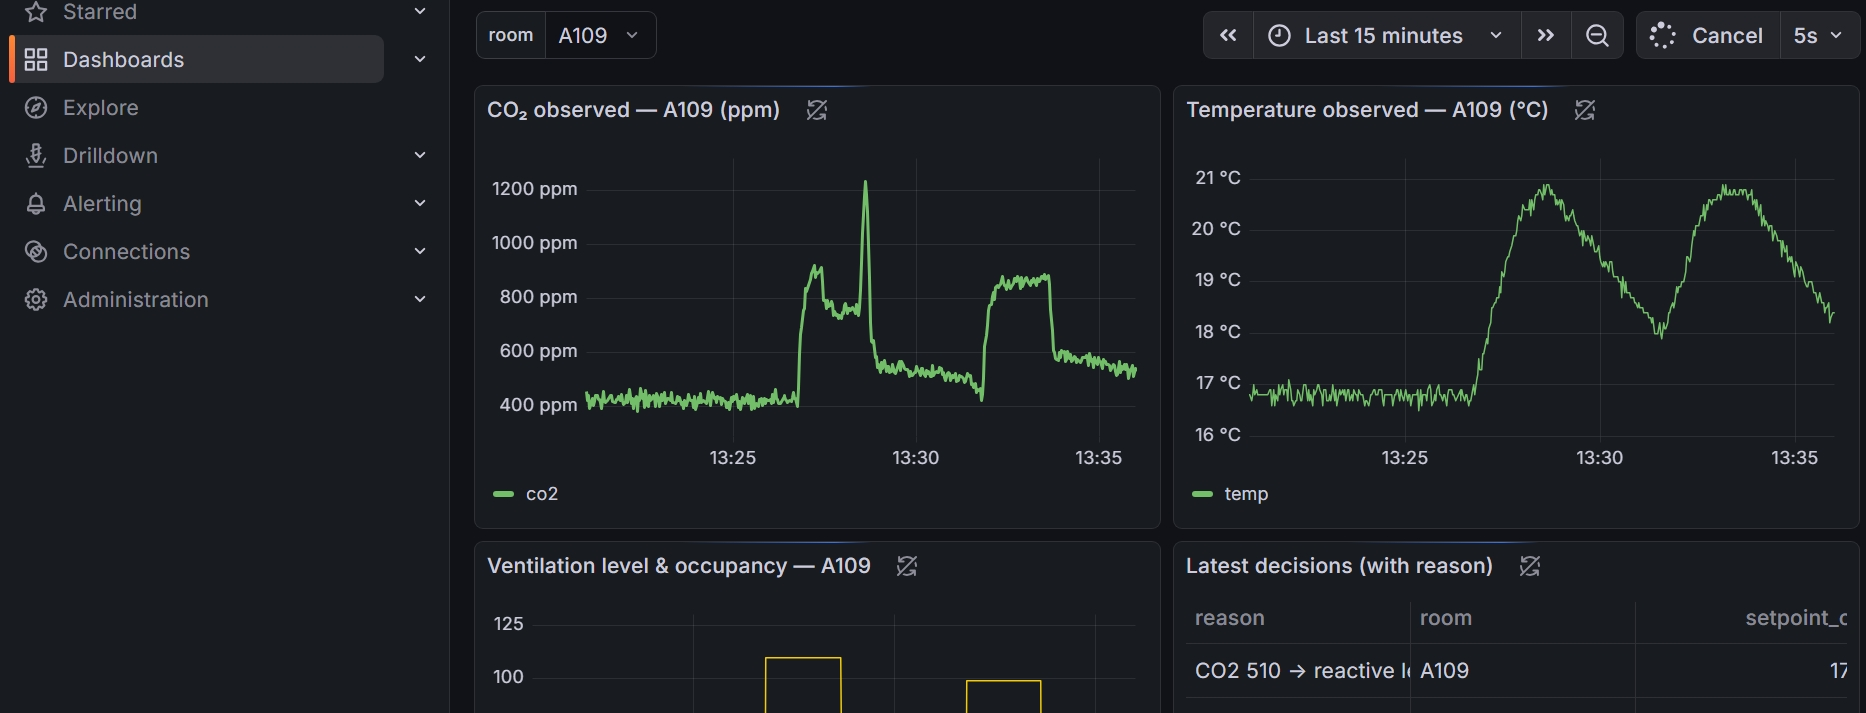
\includegraphics[width=\linewidth]{grafana_pic.jpeg}
    \caption{Grafana dashboard for A109, preserved from the supplied source document. The screenshot illustrates the presentation interface; its run provenance is unspecified.}
    \label{fig:grafana-dashboard}
\end{figure}

\section{Risks and critical reflection}
\paragraph{Physical capacity and modelling limits.}
Perfect mixing, ideal occupancy counts, fixed parameters and synthetic weather simplify reasoning but limit transfer to a real building. Inter-room air exchange, solar gains, humidity, fan electricity and active cooling are absent. Heat recovery and AHU heating are now explicit; their efficiencies and capacities are assumptions. The daily weather phase is reversed. Proportional heating may settle below setpoint, and the 19 $^\circ$C initial state plus setback makes preheating duration consequential. Modelled kWh is a comparative quantity, not metered building consumption.

For steady occupancy and constant flow,
\begin{equation}
C_{\mathrm{eq}}=C_o+\frac{10^6gn}{Q},\qquad
n_{\max}=\frac{Q(1000-C_o)}{10^6g}.
\end{equation}
At the current maximum 11 ACH, approximate steady-state occupancy bounds at 1000 ppm are 192 persons in A109, 219 in A117, 127 in A110, 17 in A323 and 16 in A113C. These analytical bounds replace the older weaker-flow values. They assume ideal mixing and steady operation, not actuator delay or arrival transients, and are neither measured nor regulatory capacities. Persistence's area-based caps can still underpredict registered crowds even when the configured airflow is physically sufficient.

\paragraph{Quality and recovery gaps.}
At factor 60, eight identical two-second-wall sensor samples span at least 14 sim-min from the first frozen publication, before control delay. Thus NFR-05's ten-minute target is inconsistent with the configured detector. Drift and implausible ranges are not generally detected; future command timestamps are not rejected. Occupancy loss can select empty-room heating, and downward-only dwell does not enforce NFR-03 for every change. A fresh plan timestamp also does not prove a fresh source sample.

The recorded F3b restart rejected an old retained command, while unchanged controller targets are not refreshed. Missing acknowledgement and reconciliation therefore threaten NFR-02. Broker queues, periodic persistence and the absence of producer outboxes limit no-loss claims. Time/receipt-window history filters fix the observed replay bug but do not fully isolate runs. The network permits truth API access even though control/planner do not use it; the architectural separation is not enforced security.

{\small\begin{longtable}{p{36mm}p{52mm}p{56mm}}\toprule Risk & Consequence & Next mitigation\\\midrule\endhead
Frozen/drifting/stale observations & Late fallback or wrong demand & Elapsed-time detection, newest-sample checks, plausibility and residual monitoring.\\
Retained command and no acknowledgement & Restarted device retains wrong state & Periodic fresh target refresh and reached-state reconciliation.\\
Timetable attendance assumption & Unnecessary heating or missed unscheduled demand & Attendance uncertainty and observed-occupancy correction; improve fika handling.\\
Shared broker, BuildSim and host & Correlated room failures & Measure outage behaviour; separate process from host redundancy claims.\\
Cross-run history and duplicates & Wrong forecasts or biased metrics & Run/session/event IDs and partitioned queries.\\
Growing file scans and storage & Query latency and memory growth & Retention bounds and incremental partitioned compaction.\\
Uncalibrated heat/energy model & Misleading comfort or energy comparison & Correct weather, calibrate and record radiator/AHU energy durably.\\
Unauthenticated lab APIs/topics & Spoofed commands, fault injection, unrestricted queries & Authentication, ACLs, TLS and narrower query access before broader use.\\\bottomrule\end{longtable}}

\paragraph{Accepted trade-offs.}
Independent device containers support isolated faults at a resource cost. MQTT offers decoupled fan-out and latest-value retention, while requiring shared-broker recovery and duplicate handling. JSONL/Parquet keeps evidence transparent without a database server, but full scans/rebuilds become expensive. A rule controller plus advisory planner keeps precedence explainable and allows history failure without stopping reactive control; it lacks joint comfort/energy optimisation.

Planning improved air quality and lecture comfort in the recorded final scenario at about 9\% more heat energy than reactive-only. High advice can also remain accepted for 60 sim-min and consume unnecessary heat. Timetable simplicity proved more useful than the rejected learned model under this simulator, but its attendance assumptions limit generalisation. More conservative sensor detection reduces delay at the cost of false alarms on stable rounded values. None of these choices removes physical capacity limits or establishes the unmeasured failure guarantees.

\paragraph{Next steps.}
First address concrete quality and recovery gaps: elapsed-time frozen detection, source freshness/range/future-time checks, command refresh and reached-state reconciliation. Introduce run/session/event identity to isolate replay windows and deduplicate retransmissions; archive timestamped radiator and AHU power/energy before physics resets.

Next improve comfort and decision quality: extend timetable-driven preheating, use observed temperature in heat decisions, retune reactive hysteresis as a simpler comparator, and improve unscheduled fika demand. Correct weather phase, calibrate thermal/flow parameters and make rollout actuator travel consistent with the simulated clock. Align training/inference aggregation and compare attendance-aware forecasts against persistence on independent dates and seeds before deployment.

Finally complete the outstanding evidence when experimentation is authorised: fixed-schedule energy comparison, repeated matched weekdays, episode-level CO\textsubscript{2} recovery, setback timing, fault/restart recovery, loss checks and scaling to a breaking point. Preserve configuration, seed, model version and run windows with every result. The existing evidence supports a conditional lecture-room improvement; comfort, unscheduled rooms and operational guarantees remain priorities.

\section*{Evidence and submission status}\addcontentsline{toc}{section}{Evidence and submission status}
The report reflects main commit \texttt{66e0805} and the identified additions on \texttt{origin/tobias} at \texttt{270d623}. Existing run artifacts and recorded live fault tests support the stated results. The supplied dashboard screenshot is preserved as interface evidence. No new application experiments were run for this revision.

\clearpage
\section*{Additional recorded evidence figures}\addcontentsline{toc}{section}{Additional recorded evidence figures}
Figures below are checked-in plots from commit \texttt{fbb5552}; they are not new experiments.
\begin{figure}[H]\centering
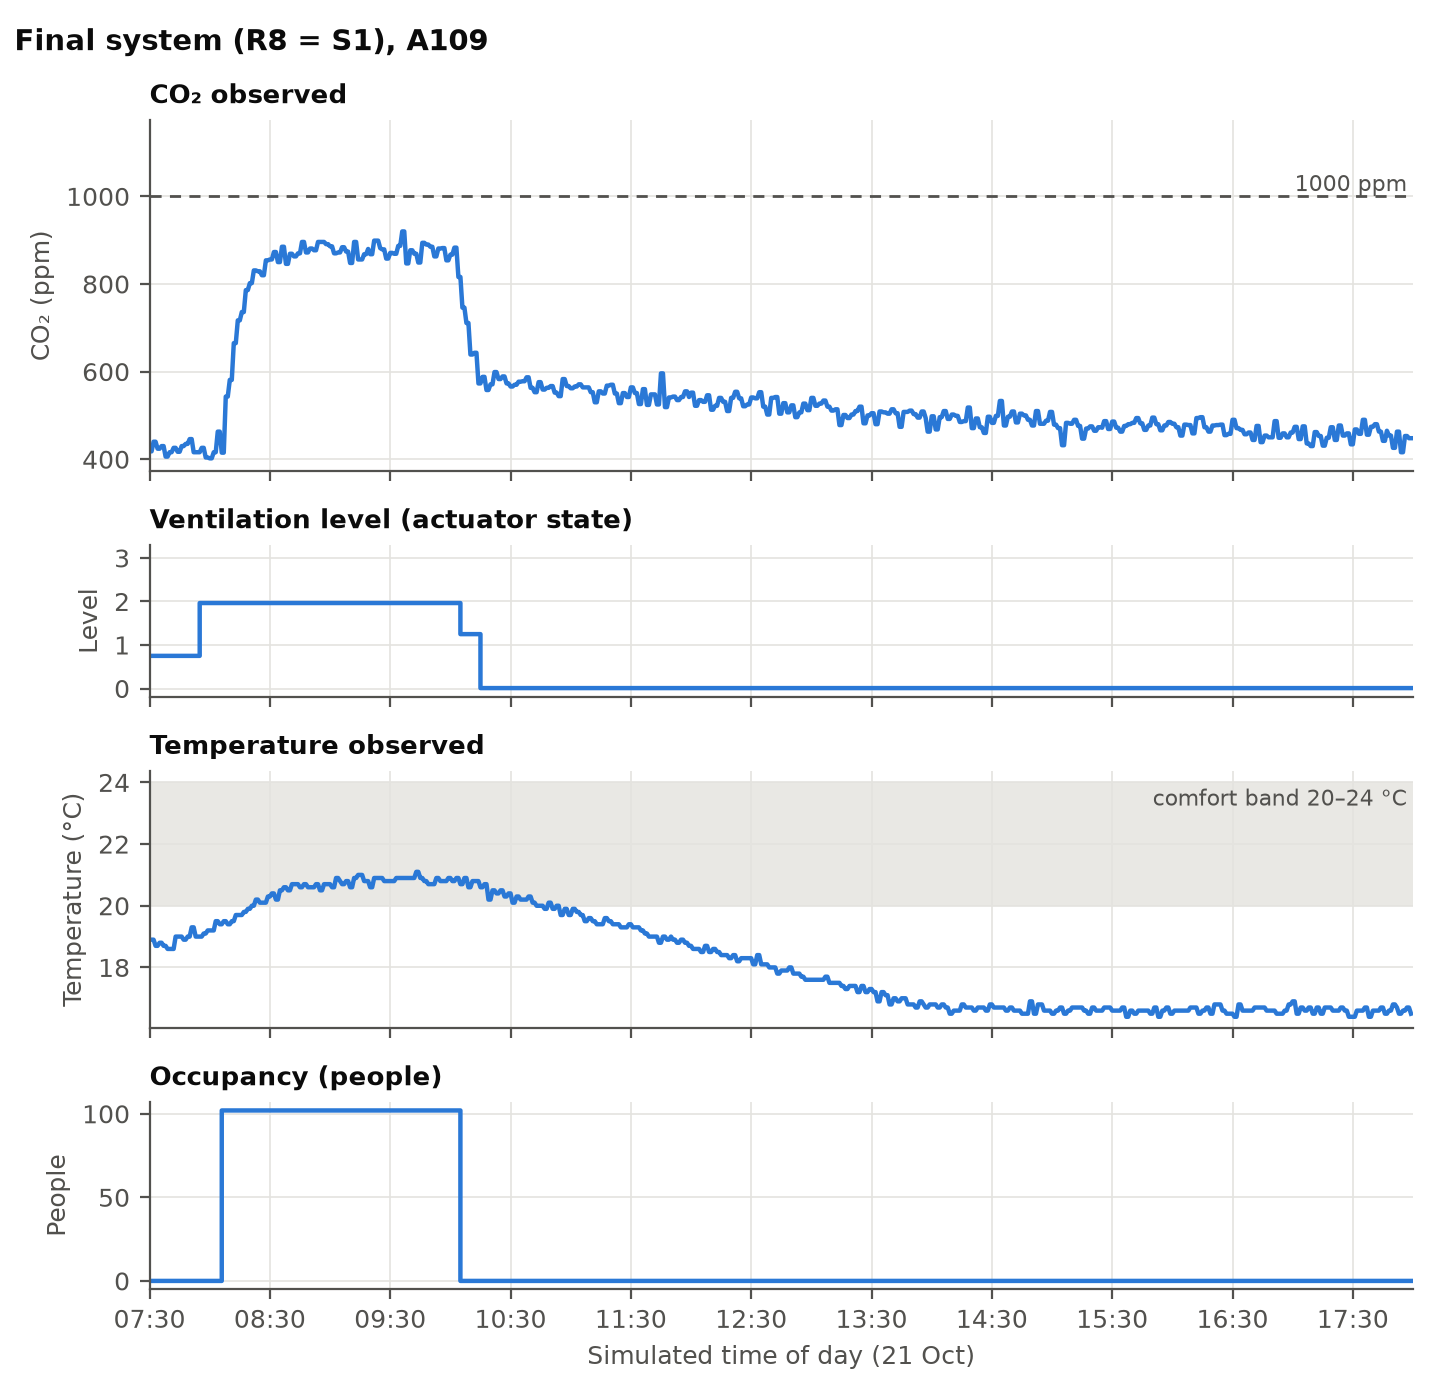
\includegraphics[width=\linewidth,height=0.78\textheight,keepaspectratio]{s1_A109.png}
\caption{Recorded A109 weekday conditions and control.}\end{figure}
\begin{figure}[H]\centering
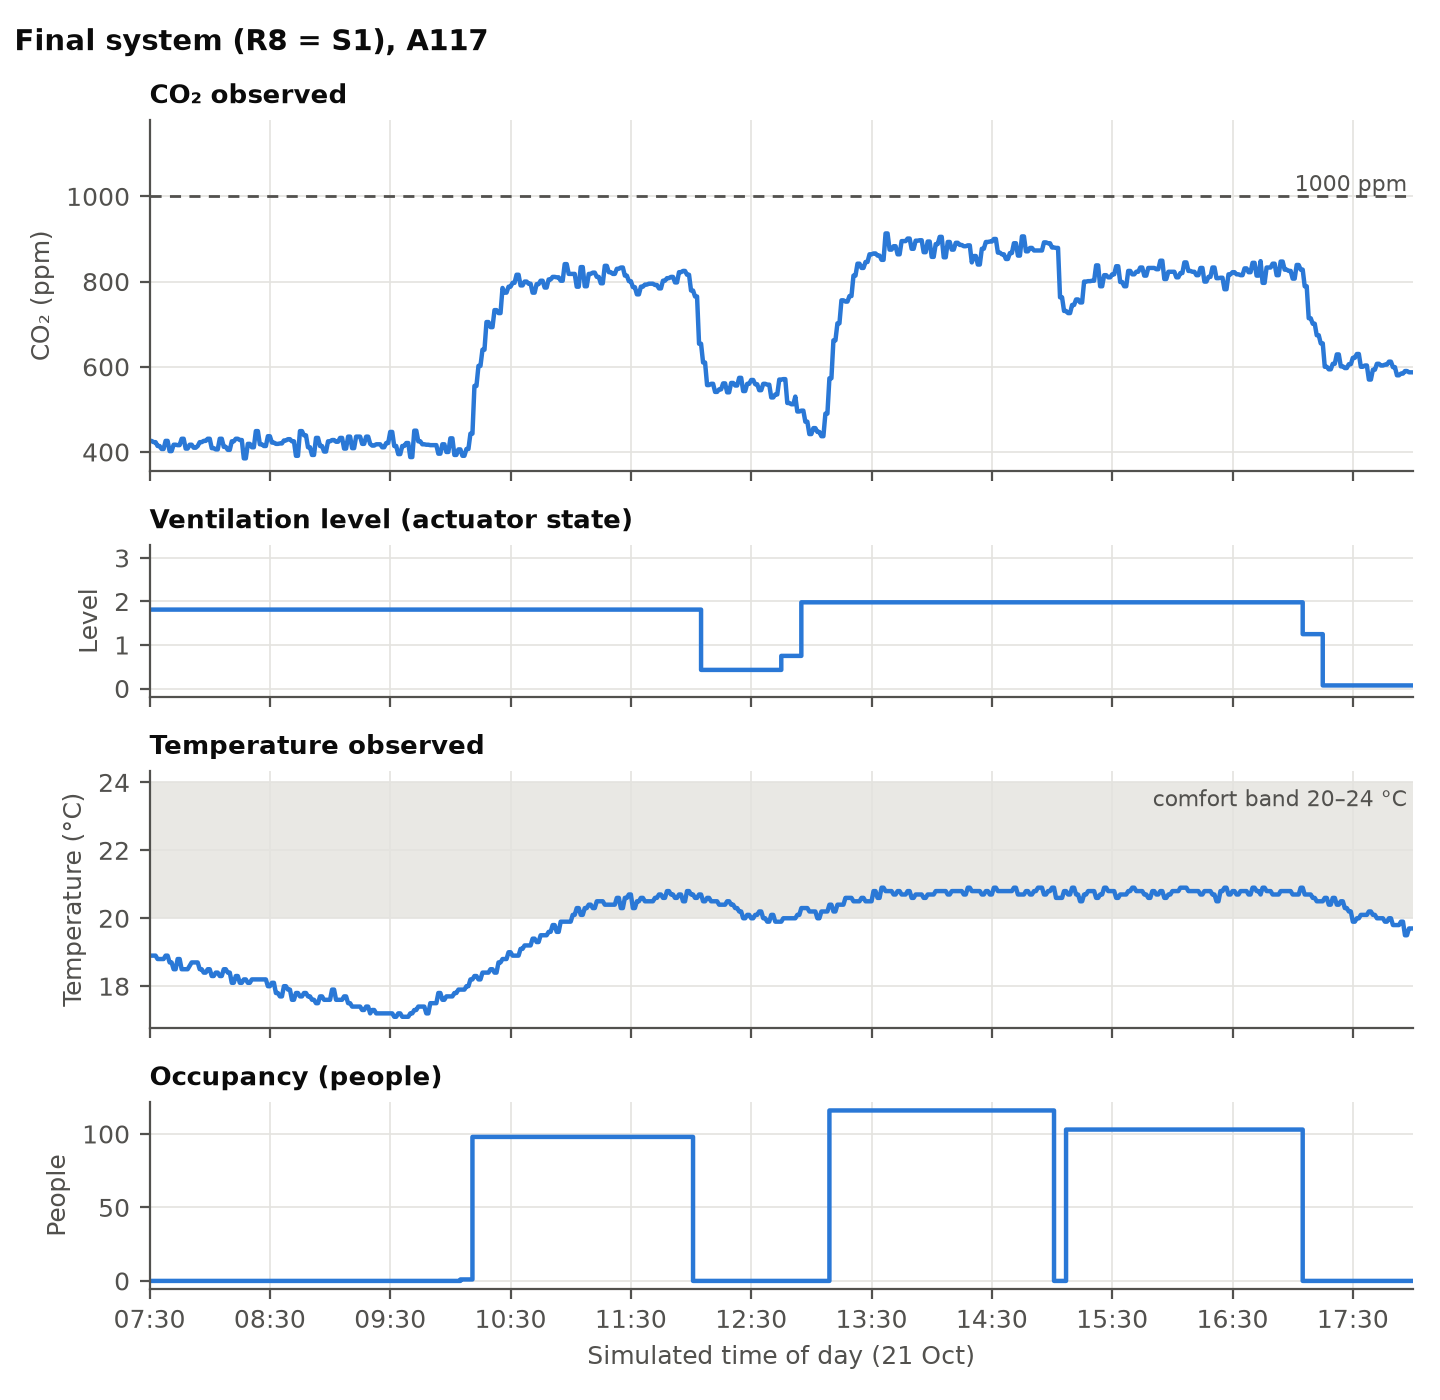
\includegraphics[width=\linewidth,height=0.78\textheight,keepaspectratio]{s1_A117.png}
\caption{Recorded A117 weekday conditions and control.}\end{figure}
\begin{figure}[H]\centering
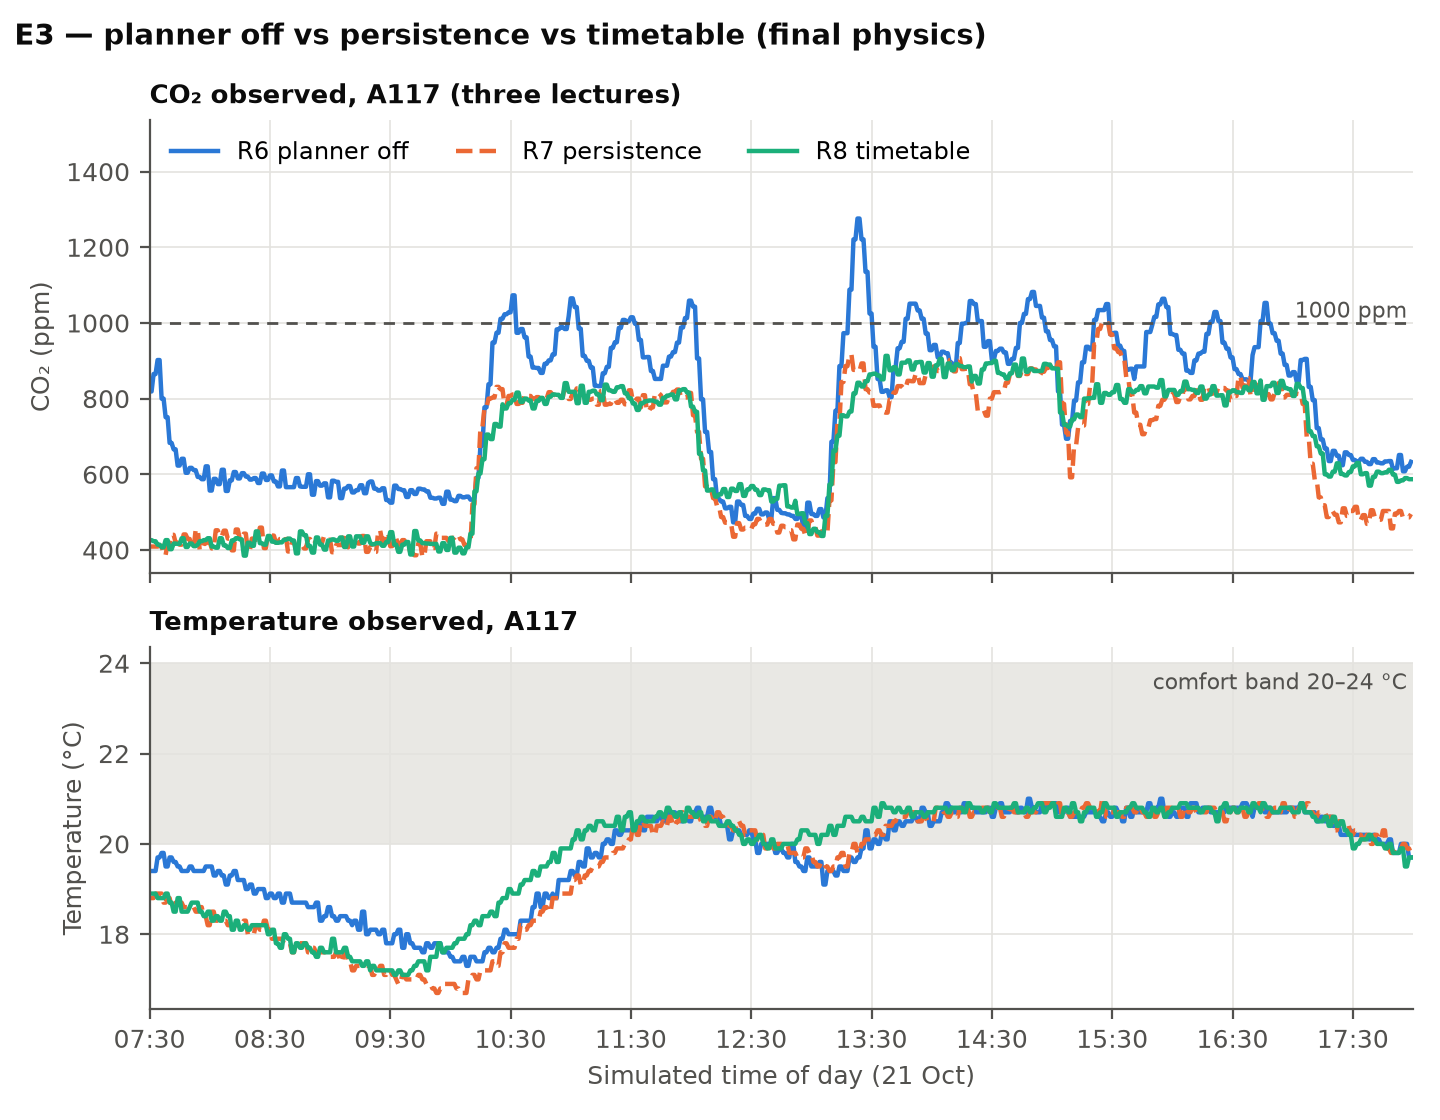
\includegraphics[width=\linewidth,height=0.78\textheight,keepaspectratio]{e3_planner_A117.png}
\caption{Recorded A117 planner comparison.}\end{figure}
\begin{figure}[H]\centering
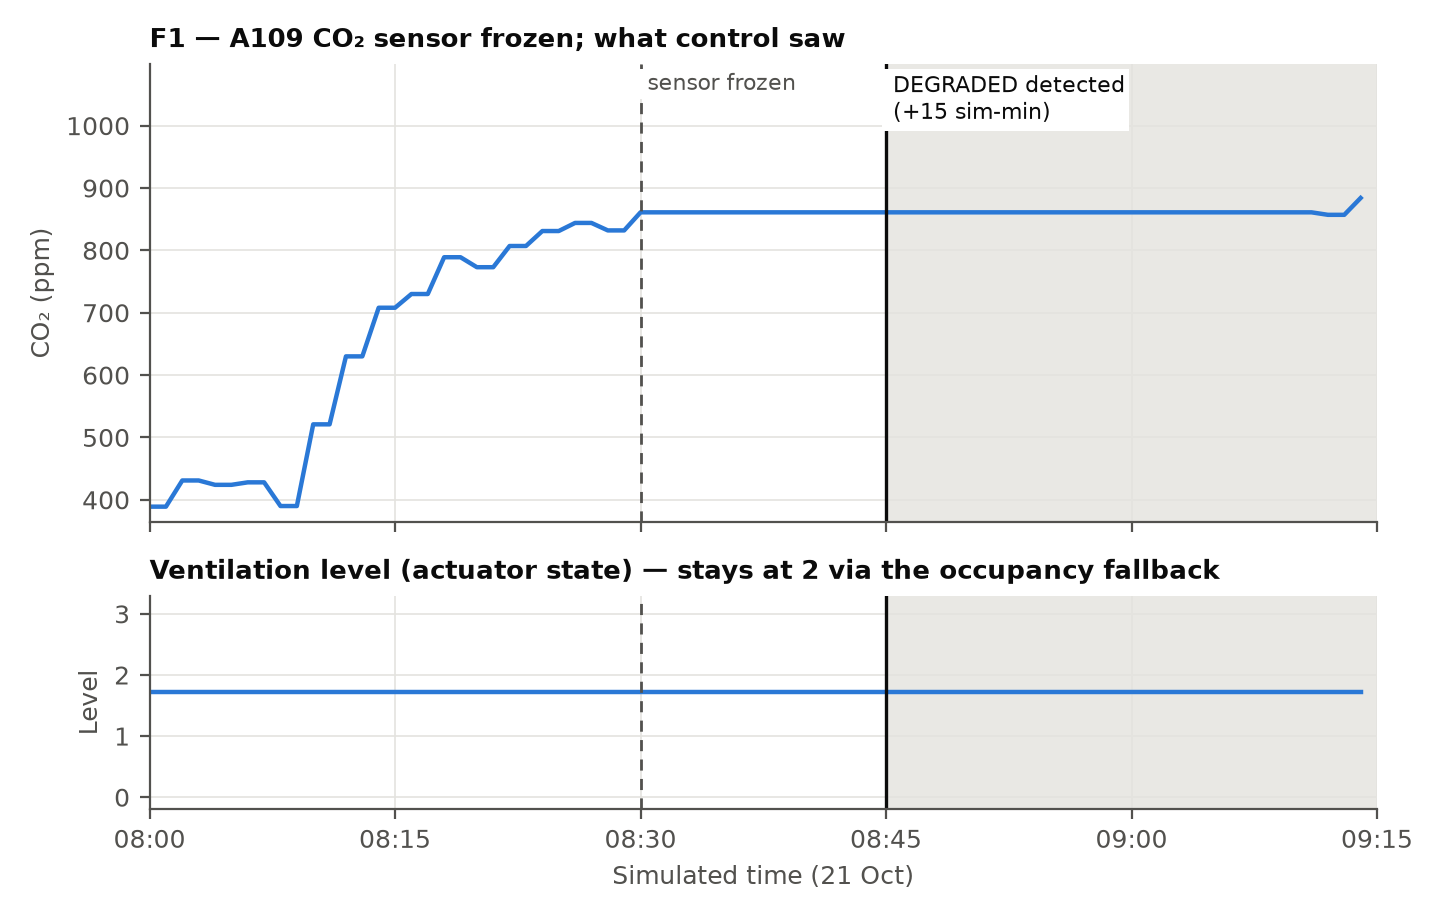
\includegraphics[width=\linewidth,height=0.78\textheight,keepaspectratio]{f1_frozen_sensor.png}
\caption{Recorded frozen-sensor test and controller fallback.}\end{figure}
\clearpage
\end{document}
